\documentclass[12pt,a4paper]{article}

% Packages nécessaires pour la charte graphique
\usepackage[utf8]{inputenc}
\usepackage[T1]{fontenc}
\usepackage[default]{lato}
\usepackage[french]{babel}
\usepackage{pdfpages}
\usepackage{xcolor}
\usepackage{titling}
\usepackage{hyperref}
\usepackage{graphicx}
\usepackage{float}
\usepackage{lastpage}
\usepackage{fancyhdr}
\usepackage{listings}
\usepackage{color}
\usepackage{geometry}
\usepackage{listings}
\usepackage{xcolor}
\usepackage{amsmath}

\edef\restoreparindent{\parindent=\the\parindent\relax}
\usepackage{parskip}
\restoreparindent


% Configuration des marges
\geometry{
  left=2cm,
  right=2cm
}

% Configuration graphicx
\graphicspath{ {./figures} }

\setlength{\headheight}{16pt}% hauteur de l'en-tête
\pagestyle{fancy}
\fancyhead{}
\fancyfoot{}
\fancyhead[L]{\thetitle}%
\fancyhead[R]{\rightmark}
\fancyfoot[R]{Page \thepage\ sur \pageref{LastPage}}%erreur d'espace à régler sur cette ligne
\fancyfoot[L]{\theauthor}
\renewcommand{\headrulewidth}{0.9pt}%trait horizontal pour l'en-tête
\renewcommand{\footrulewidth}{0.4pt}%trait horizontal pour le pied de page

% Configuration des couleurs
\definecolor{imtblue}{RGB}{0, 51, 102}
\definecolor{imtgray}{RGB}{100, 100, 100}

\lstset{
    basicstyle=\footnotesize,
    backgroundcolor=\color{gray!10!white},   
    breaklines=true,
    numbers=left,
    stepnumber=1,
}

\lstset{
    inputencoding = utf8,  % Input encoding
    extendedchars = true,  % Extended ASCII
    literate      =        % Support additional characters
      {á}{{\'a}}1  {é}{{\'e}}1  {í}{{\'i}}1 {ó}{{\'o}}1  {ú}{{\'u}}1
      {Á}{{\'A}}1  {É}{{\'E}}1  {Í}{{\'I}}1 {Ó}{{\'O}}1  {Ú}{{\'U}}1
      {à}{{\`a}}1  {è}{{\`e}}1  {ì}{{\`i}}1 {ò}{{\`o}}1  {ù}{{\`u}}1
      {À}{{\`A}}1  {È}{{\`E}}1  {Ì}{{\`I}}1 {Ò}{{\`O}}1  {Ù}{{\`U}}1
      {ä}{{\"a}}1  {ë}{{\"e}}1  {ï}{{\"i}}1 {ö}{{\"o}}1  {ü}{{\"u}}1
      {Ä}{{\"A}}1  {Ë}{{\"E}}1  {Ï}{{\"I}}1 {Ö}{{\"O}}1  {Ü}{{\"U}}1
      {â}{{\^a}}1  {ê}{{\^e}}1  {î}{{\^i}}1 {ô}{{\^o}}1  {û}{{\^u}}1
      {Â}{{\^A}}1  {Ê}{{\^E}}1  {Î}{{\^I}}1 {Ô}{{\^O}}1  {Û}{{\^U}}1
      {œ}{{\oe}}1  {Œ}{{\OE}}1  {æ}{{\ae}}1 {Æ}{{\AE}}1  {ß}{{\ss}}1
      {ẞ}{{\SS}}1  {ç}{{\c{c}}}1 {Ç}{{\c{C}}}1 {ø}{{\o}}1  {Ø}{{\O}}1
      {å}{{\aa}}1  {Å}{{\AA}}1  {ã}{{\~a}}1  {õ}{{\~o}}1 {Ã}{{\~A}}1
      {Õ}{{\~O}}1  {ñ}{{\~n}}1  {Ñ}{{\~N}}1  {¿}{{?`}}1  {¡}{{!`}}1
      {°}{{\textdegree}}1 {º}{{\textordmasculine}}1 {ª}{{\textordfeminine}}1
      {£}{{\pounds}}1  {©}{{\copyright}}1  {®}{{\textregistered}}1
      {«}{{\guillemotleft}}1  {»}{{\guillemotright}}1  {Ð}{{\DH}}1  {ð}{{\dh}}1
      {Ý}{{\'Y}}1    {ý}{{\'y}}1    {Þ}{{\TH}}1    {þ}{{\th}}1    {Ă}{{\u{A}}}1
      {ă}{{\u{a}}}1  {Ą}{{\k{A}}}1  {ą}{{\k{a}}}1  {Ć}{{\'C}}1    {ć}{{\'c}}1
      {Č}{{\v{C}}}1  {č}{{\v{c}}}1  {Ď}{{\v{D}}}1  {ď}{{\v{d}}}1  {Đ}{{\DJ}}1
      {đ}{{\dj}}1    {Ė}{{\.{E}}}1  {ė}{{\.{e}}}1  {Ę}{{\k{E}}}1  {ę}{{\k{e}}}1
      {Ě}{{\v{E}}}1  {ě}{{\v{e}}}1  {Ğ}{{\u{G}}}1  {ğ}{{\u{g}}}1  {Ĩ}{{\~I}}1
      {ĩ}{{\~\i}}1   {Į}{{\k{I}}}1  {į}{{\k{i}}}1  {İ}{{\.{I}}}1  {ı}{{\i}}1
      {Ĺ}{{\'L}}1    {ĺ}{{\'l}}1    {Ľ}{{\v{L}}}1  {ľ}{{\v{l}}}1  {Ł}{{\L{}}}1
      {ł}{{\l{}}}1   {Ń}{{\'N}}1    {ń}{{\'n}}1    {Ň}{{\v{N}}}1  {ň}{{\v{n}}}1
      {Ő}{{\H{O}}}1  {ő}{{\H{o}}}1  {Ŕ}{{\'{R}}}1  {ŕ}{{\'{r}}}1  {Ř}{{\v{R}}}1
      {ř}{{\v{r}}}1  {Ś}{{\'S}}1    {ś}{{\'s}}1    {Ş}{{\c{S}}}1  {ş}{{\c{s}}}1
      {Š}{{\v{S}}}1  {š}{{\v{s}}}1  {Ť}{{\v{T}}}1  {ť}{{\v{t}}}1  {Ũ}{{\~U}}1
      {ũ}{{\~u}}1    {Ū}{{\={U}}}1  {ū}{{\={u}}}1  {Ů}{{\r{U}}}1  {ů}{{\r{u}}}1
      {Ű}{{\H{U}}}1  {ű}{{\H{u}}}1  {Ų}{{\k{U}}}1  {ų}{{\k{u}}}1  {Ź}{{\'Z}}1
      {ź}{{\'z}}1    {Ż}{{\.Z}}1    {ż}{{\.z}}1    {Ž}{{\v{Z}}}1
      % ¿ and ¡ are not correctly displayed if inconsolata font is used
      % together with the lstlisting environment. Consider typing code in
      % external files and using \lstinputlisting to display them instead.      
  }


% Configuration du titre
\renewcommand{\maketitle}{
  \begin{center}
    {\huge\color{imtblue}\thetitle} \\[1em]
    \theauthor \\[1em]
    \today \\[1em]
    \hrule
  \end{center}
}

% Configuration des hyperliens
\hypersetup{
    colorlinks=true,
    linkcolor=imtblue,
    filecolor=imtblue,      
    urlcolor=imtblue,
}


% FIN DE LA CONFIGURATION - DEBUT DU DOCUMENT

\title{SIT213 : Livrable}
\author{Rayane BELKHIR, Tchadel ICARD, Alexis FUCHS, Dan ACHILLE, Lia ALEGRE}
\date{\today}


\begin{document}

\thispagestyle{empty} % Supprime le numéro de page de cette page

\vspace*{\fill} % Ajoute de l'espace vertical élastique
\maketitle
\vspace*{\fill} % Ajoute de l'espace vertical élastique

\newpage
\tableofcontents
\newpage

\listoffigures

\section*{Introduction}
\sectionmark{Introduction}
\addcontentsline{toc}{section}{Introduction}

Le but de ce livrable est de rendre compte des résultats des simulations effectués tout au long du projet, et comparer ceux-ci aux résultats théoriques attendus pour chacun des cas d'usage.

En plus d'aborder le thème des télécommunication, il s'agit aussi de réaliser des tests unitaires, pour valider la conformité de notre code tout au long du développement, et éviter, notamment, les régressions lors de changements sur du code déjà validé.

Chaque partie de ce rapport correspond ainsi à une étape (1 livrable) de notre projet.

\section{TP1 : Transmission "back-to-back" - Mise en place de l'infrastructure}
\sectionmark{TP1 : Transmission "back-to-back" - Mise en place de l'infrastructure}

Cette étape est la première de ce projet, nous ayant permis de prendre en main l'architecture logicielle et des livrables à prévoir.

La transmission est, dans ce premier livrable, parfaite. Le calcul du T-E-B est donc pour l'instant inutile (malgré qu'il ait été implémenté), puisque toujours égal à 0 dans cette étape quelles que soit les conditions.

\begin{figure}[H]
    \centering
    
\includegraphics[width=\textwidth]{img/teb1.jpg}
    \caption{Taux d'erreur binaire pour une source aléatoire de 100 bits}
    \label{fig:teb1}
\end{figure}
\begin{figure}[H]
    \centering
    
\includegraphics[width=\textwidth]{img/teb3.jpg}
    \caption{Taux d'erreur binaire pour une source aléatoire avec seed}
    \label{fig:teb2}
\end{figure}
\begin{figure}[H]
    \centering
    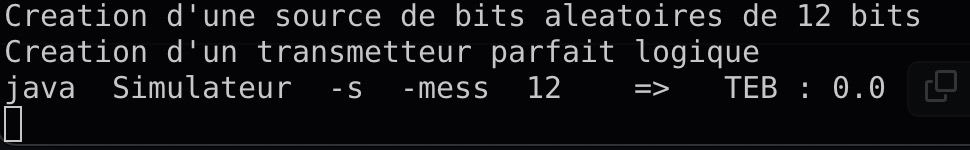
\includegraphics[width=\textwidth]{img/teb2.jpg}
    \caption{Taux d'erreur binaire pour une source fixé par l'utilisateur}
    \label{fig:teb3}
\end{figure}
\begin{figure}[H]
    \centering
    
\includegraphics[width=\textwidth]{img/teb4.jpg}
    \caption{Taux d'erreur binaire pour une source fixé par l'utilisateur (en binaire)}
    \label{fig:teb4}
\end{figure}


Ainsi on observe dans les 4 cas :
\begin{itemize}
    \item Message liés à la génération de 100 symboles aléatoires à l'exécution ;
    \item Message liés à la génération de 100 symboles aléatoires à partir d'une seed fixée par l'utilisateur (\texttt{-seed [chaîne de caractères]}) ;
    \item Message fixés par l'utilisateur (\texttt{-mess [chaîne de caractères]}) ;
\end{itemize}

que le résultat de la transmission dans notre simulation est l'exact réplique de la source.

\begin{figure}[H]
    \centering
    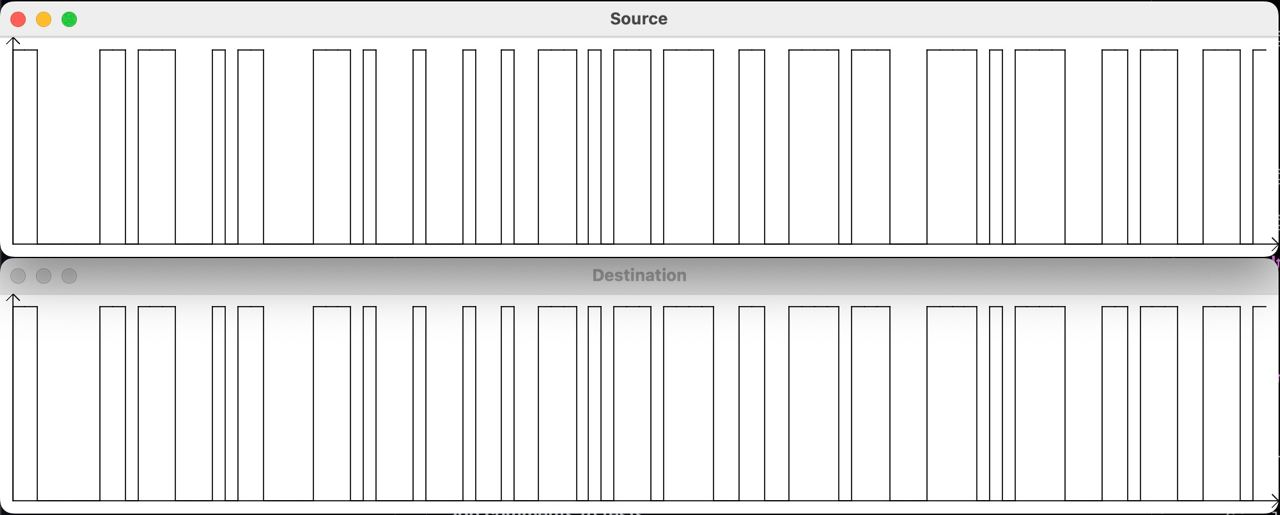
\includegraphics[width=\textwidth]{img/source_et_dest.jpg}
    \caption{Résultat d'une simulation entre source et destination}
    \label{fig:simulation1}
\end{figure}

Nos sondes ont été, en effet, placés en sortie de la source, ainsi qu'en sortie du transmetteur parfait (juste avant la destination finale).

Les résultats de la simulation correspondent bien aux attentes de l'énoncé et aux prévisions que l'on pouvait avoir avant la réalisation de celle-ci.





\section{TP2 : Transmission non bruitée analogique}
\sectionmark{TP2 : Transmission non bruitée analogique}

\subsection{Introduction étape 2}
Dans la continuité de l'étape 1, nous étudierons le comportement du système de transmission en tenant compte de la nature analogique du canal de transmission. Nous aborderons ainsi les différents types de codages analogiques implémentés.

\begin{figure}[H]
    \centering
    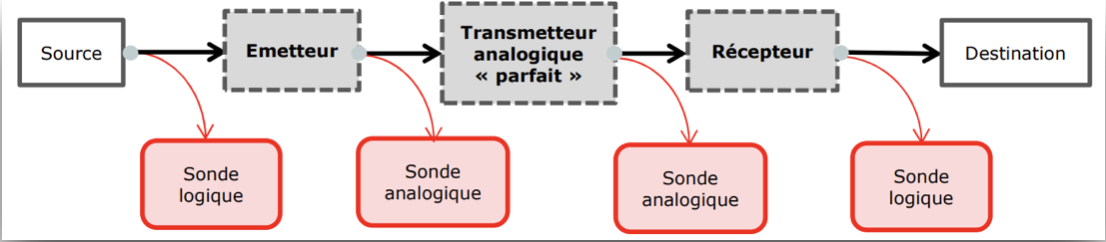
\includegraphics[width=0.7\textwidth]{img/etape2_chaine_transmission.png}
    \caption{Chaîne de transmission}
    \label{fig:chaine_transmission}
\end{figure}

\subsection{Objectifs}
Pour cette deuxième étape, nous maintenons la capacité d'envoyer un message binaire, mais avec un transmetteur analogique \textit{parfait} qui garantira toujours un TEB de 0 (puisque pas de bruit). Les nouveautés liées au transmetteur analogique incluent le choix de la forme d'onde et la spécification du nombre d'échantillons par bit ainsi que les amplitudes min et max.

\subsection{Paramètres du logiciel}
Le paramètre \texttt{form f} permet de spécifier la forme d'onde pour la transmission analogique. Les options disponibles sont :

\begin{enumerate}
    \item \textbf{NRZ} : Forme d'onde rectangulaire.
    \item \textbf{NRZT} : Forme d'onde trapézoïdale (temps de montée et de descente à 1/3 du temps bit).
    \item \textbf{RZ} : Forme d'onde impulsionnelle (amplitude minimale sur le premier et dernier tiers du temps bit, impulsionnelle sur le tiers central avec un maximum au milieu du temps bit égal à l'amplitude maximale).
\end{enumerate}

Par défaut, le simulateur utilise la forme d'onde RZ pour le signal analogique.

Le paramètre \texttt{nbEch ne} permet de spécifier le nombre d'échantillons par bit dans la transmission analogique. Il doit être une valeur entière positive. Par défaut, le simulateur utilise 30 échantillons par bit.

Le paramètre \texttt{ampl min max} spécifie l'amplitude minimale et maximale du signal analogique. Ils doivent être des valeurs flottantes, avec min < max. Par défaut, le simulateur utilise 0.0f comme valeur minimale et 1.0f comme valeur maximale.

\subsection{Réalisation}
Pour la gestion de projet, nous avons opté pour l'outil Taiga. Cet outil nous permet de définir les tâches attribuées à chaque membre de l'équipe, d'organiser la planification et de prioriser lesdites tâches, ainsi que de suivre leurs avancements. 

\begin{figure}[H]
    \centering
    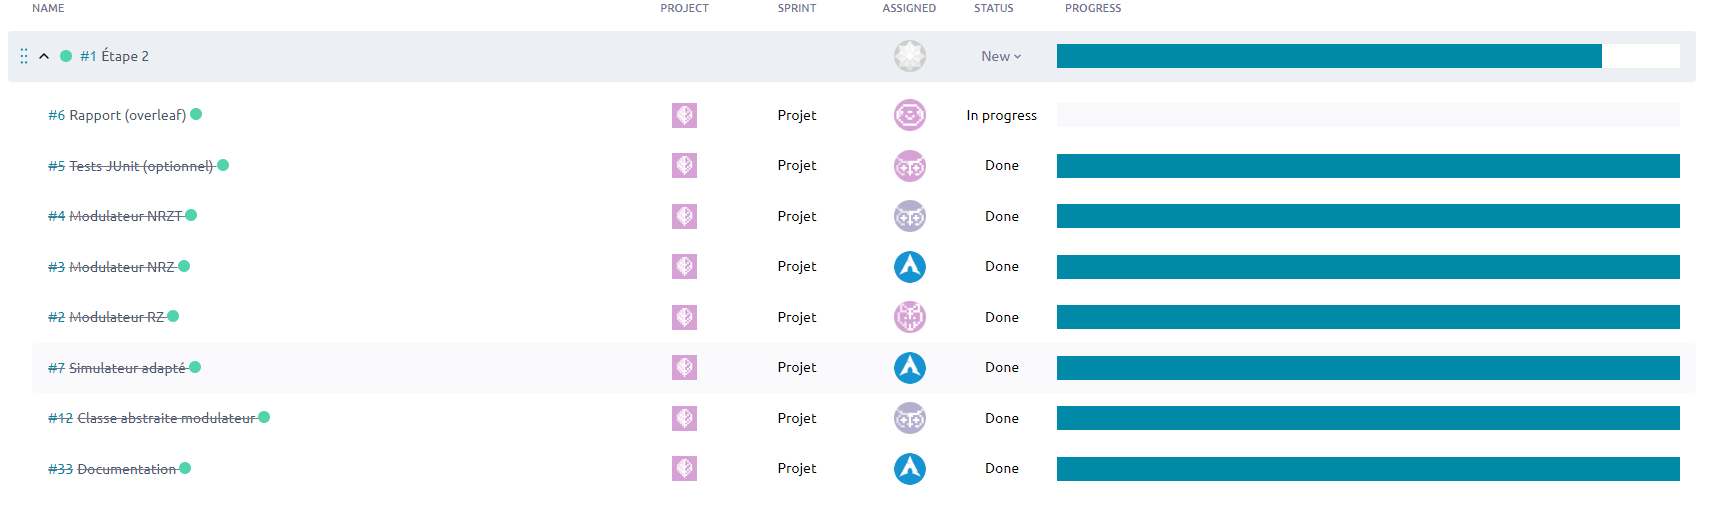
\includegraphics[width=1\textwidth]{img/etape2_taiga.png}
    \caption{Liste des tâches (divisées en sous-tâches) dans Taiga}
    \label{fig:etape2_taiga}
\end{figure}

En ce qui concerne le développement logiciel, nous utilisons un dépôt Git sur GitHub. Cette approche permet à tous les membres de l'équipe d'accéder facilement au code et assure une traçabilité de toutes les versions.


\subsection{Émetteur analogique}
Dans notre contexte de chaîne de transmission analogique, nous avons établit que nous devions faire la chaîne de transmission par l’adjonction de deux étages (logique → analogique et analogique → logique). Pour ce faire, nous allons tout d’abord nous intéresser à l’émission de notre signal. 

Dans notre code, les classes \textbf{Emetteur} et \textbf{Recepteur} doivent être modifiées pour gérer l’emission analogique. Notamment la prise en charge de trois formes d’ondes: NRZ, NRZT et RZ. Chaque type d’onde aura une méthode dédiée qui nous permettra de réaliser son traitement.

\subsubsection{Émission analogique NRZ}
Le codage NRZ (Non Return to Zero) permet la transmission d’un signal via un système d’échelonnage. Il représente une des manière les plus simple de transmission car il n’y a pas de niveau intermédiaire, mais seulement deux états binaire 0 et 1 :

\begin{itemize}
    \item Bit à 1 en entrée : le flottant (correspondant à la valeur du signal) prend comme valeur l’amplitude maximal $A_{max}$
    \item Bit à 0 en entrée : le flottant (correspondant à la valeur du signal) prend comme valeur l’amplitude minimal $A_{min}$
\end{itemize}

\begin{figure}[H]
    \centering
    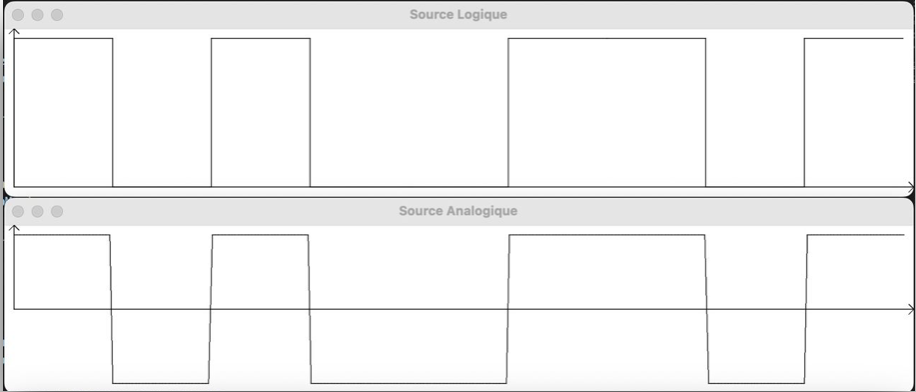
\includegraphics[width=0.5\textwidth]{img/etape2_transmission_NRZ.png}
    \caption{Transmission NRZ}
    \label{fig:transmission_nrz}
\end{figure}

On observe bien au niveau de la source analogique que pour un bit un 1 en entrée on a une amplitude d’une valeur de 1. Alors que pour une bit à 0 en entrée, on a une amplitude de -1. La figure ci-dessus illustre bien la conversion du signal logique en signal analogique, étant donnée que l’amplitude pour les 0 logiques n’est plus de 0 mais bien de -1.

\subsubsection{Émission analogique NRZT}

Le codage NRZT (NRZ Trapézoïdal) reprend le même principe que le codage NRZ. C’est à dire que l’on réalise la transmission d’un signal via un système d’échelonnage, avec deux états binaires simple et aucun  niveau intermédiaire. Ce qui diffère est le temps de montée et descente entre deux états binaires, ce qui a pour conséquence  de faire apparaître une pente au début et à la fin du bit. Du fait de ce nouveau facteur, on aura un codage différent selon selon la valeur des symboles précédents et suivants.

\begin{figure}[H]
    \centering
    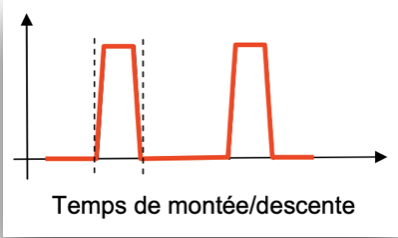
\includegraphics[width=0.33\textwidth]{img/etape2_temps_NRZT.png}
    \caption{Temps bit NRZT}
    \label{fig:emission_nrzt}
\end{figure}

D’après ce que l’on a dit précédemment, on peut en déduire que l’on va devoir utiliser des nombres flottant pour pouvoir coder la montée/descente. Cela va impacter la manière dont on code les symboles, chaque symbole pouvant être découper en 3 temps :

\begin{itemize}
    \item Le premier temps : le temps de montée du symbole (1/3 de la période)
    \item Le deuxième temps : l’amplitude Amax/Amin est atteint (1/3 de la période)
    \item Le troisième temps : le temps de la descente du symbole (1/3 de la période)
\end{itemize}

Si on rencontre le cas où il y a deux bits logiques successives de même valeur, il n’y a pas descente. La descente aura lieu au moment où la valeur du bit logique changera.

\begin{figure}[H]
    \centering
    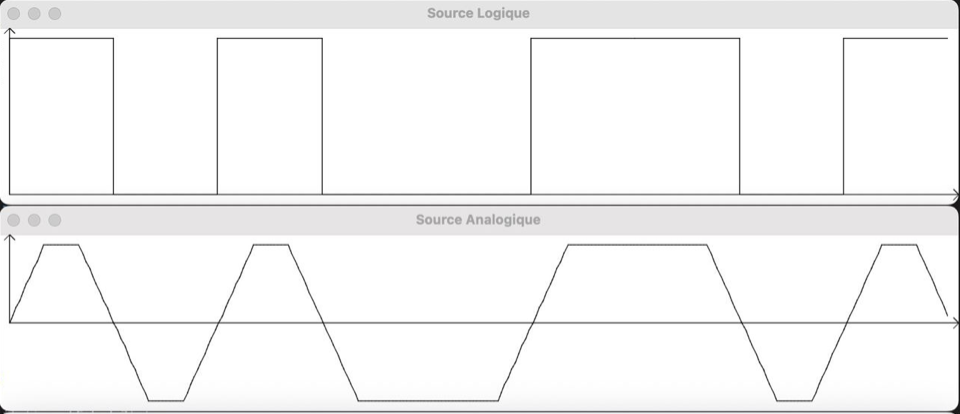
\includegraphics[width=0.5\textwidth]{img/etape2_emission_NRZT.png}
    \caption{Émission NRZT}
    \label{fig:emission_nrzt}
\end{figure}

On observe bien au niveau de la sonde analogique que le symbole est monté progressivement, de même pour la descente. Le signal varie toujours entre les deux seuil et on obtient donc bien le résultat attendu, comme on la décrit précédemment.



\subsubsection{Émission analogique RZ}

Le codage RZ (Return Zero), il s’agit aussi d’un codage à 2 niveaux. La différence entre NRZ et RZ est que dans le cas du RZ le signal retourne à la valeur 0 entre chaque bit logique codé, même dans le cas de bit logique de même valeur.

\begin{figure}[H]
    \centering
    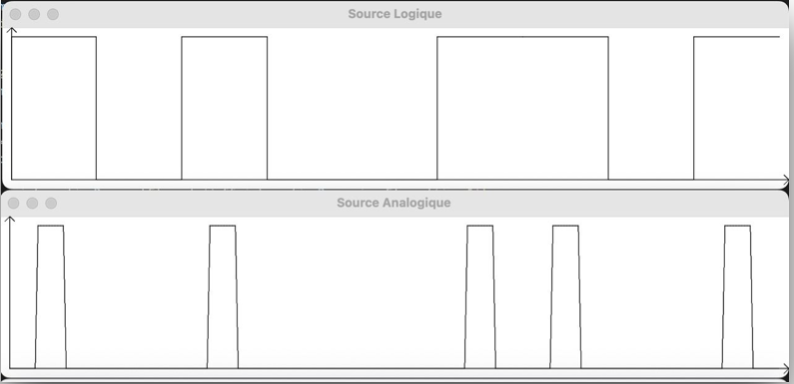
\includegraphics[width=0.5\textwidth]{img/etape2_emission_RZ.png}
    \caption{Émission RZ}
    \label{fig:emission_rz}
\end{figure}

On observe sur la figure ci-dessus, que la source analogique contient une suite de deux bit logique de valeur 1. Et une fois qu’on applique le codage RZ, on a bien deux symbole codant le bit logique 1 séparé par un seuil à 0. On a donc bien réussi à appliquer le codage RZ comme décrit précédemment.

\subsection{Récepteur analogique}

Nous allons à présent aborder la réception au sein de notre chaîne de transmission. Pour ce faire, nous devons prendre en charge les différentes méthodes de transmission que nous avons précédemment codées, à savoir :

\begin{itemize}
    \item Le NRZ (Non-Return-to-Zero)
    \item Le NRZT (Non-Return-to-Zero with Trailing Zeros)
    \item Le RZ (Return-to-Zero)
\end{itemize}

Une fois que le type de récepteur a été sélectionné, il nous faudra prendre en compte le nombre d'échantillons établis par l'émetteur. Le récepteur reçoit des données au format float et, en fonction du nombre d'échantillons précédemment choisi, il capturera la valeur et appliquera un traitement pour obtenir le codage souhaité.

La classe \textbf{Récepteur} est responsable de la gestion de la réception analogique et prend en charge les trois types de codage mentionnés (NRZ, NRZT et RZ) à travers trois méthodes distinctes, chacune traitant une forme d'onde spécifique.

\subsubsection{Réception analogique NRZ}

La réception d'un signal de type NRZ (Non-Return-to-Zero) repose sur la détection des fronts montants. Dans ce type de signal, les niveaux sont significatifs, et il n'y a pas de niveaux intermédiaires. Pour déterminer la valeur logique de ce signal, on calcule la valeur moyenne du signal analogique NRZ, qui est définie comme la moyenne entre les niveaux maximal ($A_{max}$) et minimal ($A_{min}$) du signal.

Si la valeur lue du signal analogique NRZ est supérieure à la valeur moyenne, alors on interprète cette partie du signal comme étant un 1 logique. Dans le cas contraire, lorsque la valeur est inférieure à la valeur moyenne, on la considère comme étant un 0 logique.

La figure suivante représente le signal analogique NRZ en haut et sa version logique correspondante en bas, illustrant ainsi le processus décris. Le message représenté est \texttt{101001101}.

\begin{figure}[H]
    \centering
    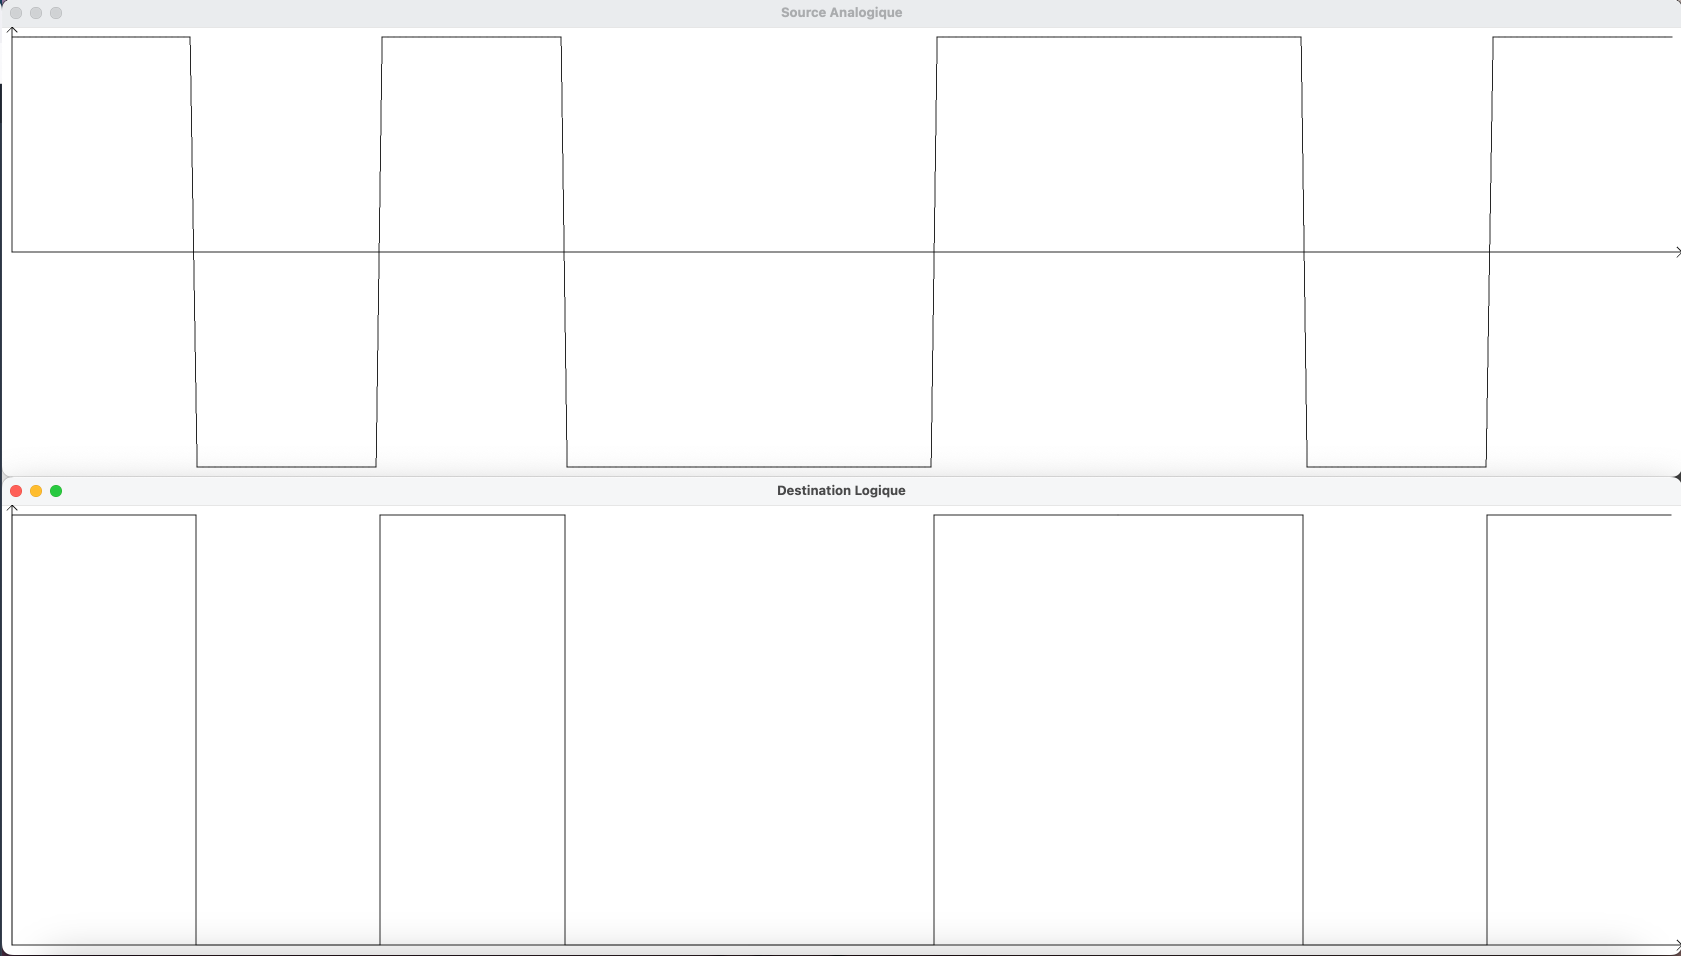
\includegraphics[width=0.5\textwidth]{img/etape2_reception_NRZ.png}
    \caption{Réception NRZ}
    \label{fig:reception_nrz}
\end{figure}

Nous pouvons constater que le message analogique émis est converti correctement. Les 0 du message transmis possèdent bien l'amplitude minimale en analogique (-1) et sont bien à 0 en numérique. Les 1, quant à eux, possèdent bien l'amplitude maximale en analogique (1) et sont bien à 1 en numérique. Le principe est similaire au transmetteur parfait, puisque seules les amplitudes sont modifiées. Par ailleurs, aucune déformation n'a été induite sur le signal. La chaine de transmission respecte les contraintes imposées, avec un TEB de 0\%.

\subsubsection{Réception analogique NRZT}

La réception d'un signal de type NRZT (Non-Return-to-Zero with Trailing Zeros) repose sur la détection de seuil, une technique spécifique qui améliore la fiabilité de la réception des données. Pour ce faire, un indice est positionné au milieu de la durée d'émission d'un bit, ce qui permet une évaluation précise de sa valeur. Cette approche est particulièrement utile pour les signaux NRZT, car elle permet de distinguer efficacement entre les valeurs 0 et 1.

Lorsque l'indice de milieu de bit est atteint, une mesure est effectuée, et la valeur résultante est comparée à un seuil prédéfini. Si la valeur mesurée est supérieure à zéro, le bit mesuré est considéré comme étant 1. En revanche, si la valeur mesurée est inférieure ou égale à zéro, le bit est fixé à 0. Cette méthode de détection de seuil permet de minimiser les erreurs de décodage, car elle tient compte de la valeur relative par rapport à un point de référence au milieu du bit.

La figure ci-dessous illustre le processus de transmission de données utilisant le codage NRZT (Non-Return-to-Zero with Trailing Zeros). En haut, vous pouvez voir un signal analogique généré par la source,  et en bas, le signal logique reçu par la destination est représenté. Le message envoyé est \texttt{101001101}. Cette représentation visuelle montre comment le signal analogique est encodé et décodé pour obtenir la séquence de bits d'origine. 

\begin{figure}[H]
    \centering
    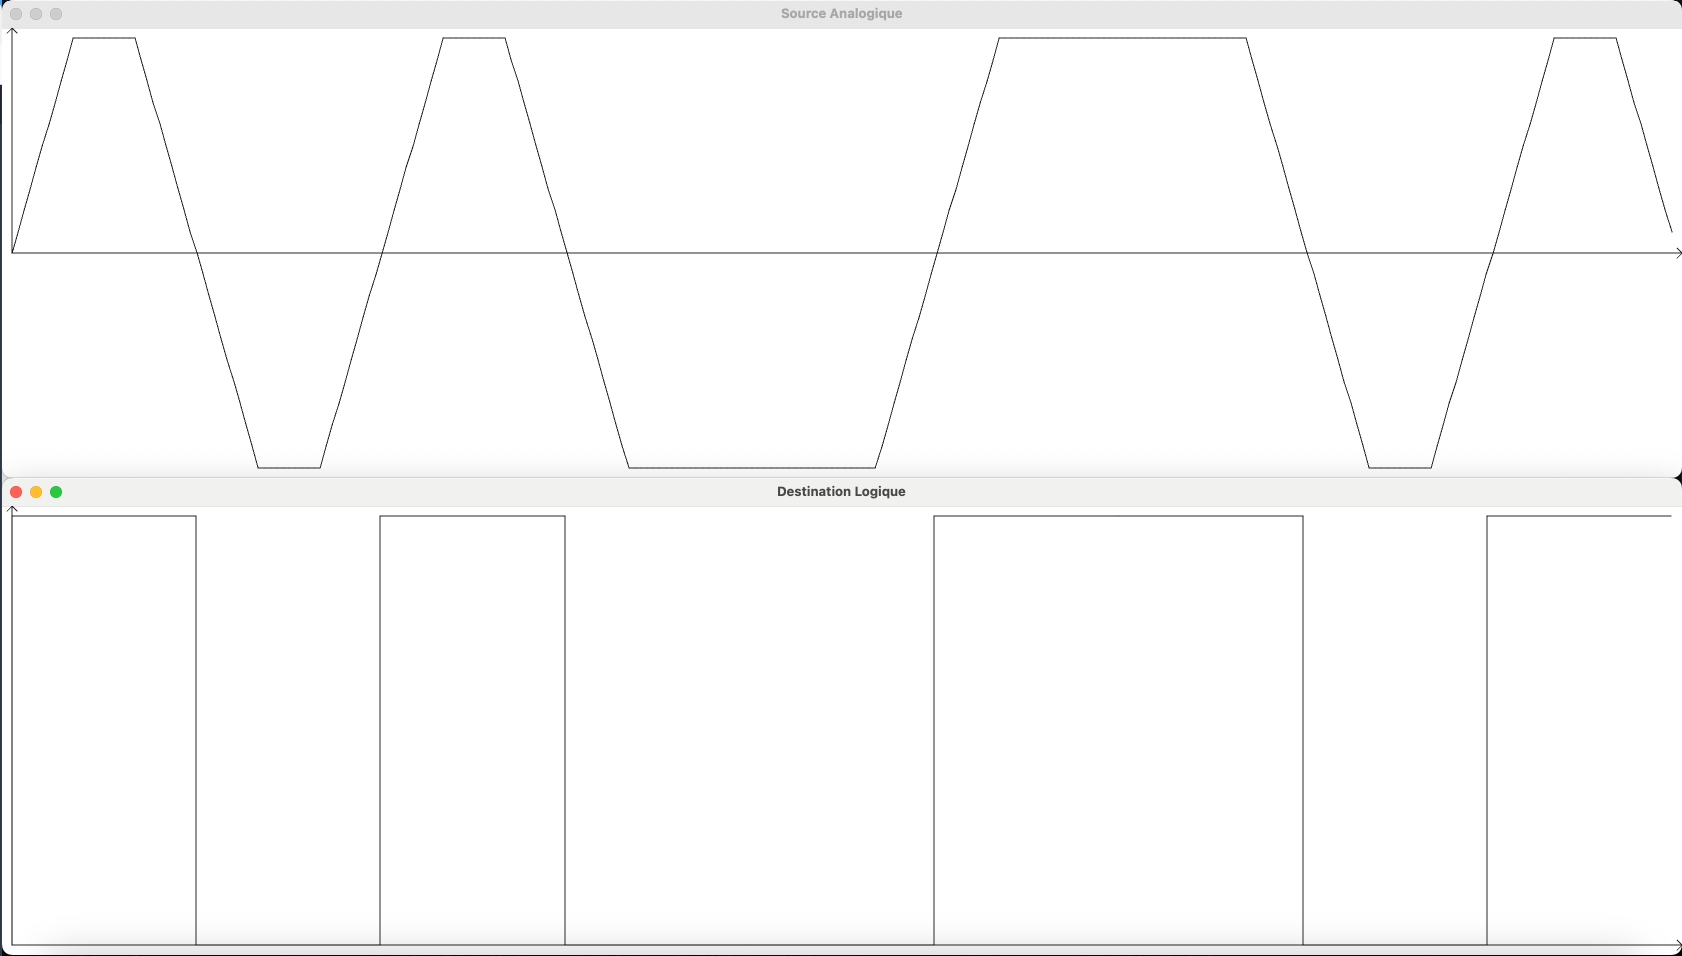
\includegraphics[width=0.5\textwidth]{img/etape2_reception_NRZT.png}
    \caption{Réception NRZT}
    \label{fig:reception_nrzt}
\end{figure}

On observe que les temps de montée et de descente correspondent bien à 1/3 du temps bit respectivement. Par ailleurs, signal n'est pas altéré, il s'agit bien d'un transmetteur analogique parfait. Le TEB est de 0\%.

\subsubsection{Réception analogique RZ}

Le codage RZ (Return-to-Zero) présente la particularité de revenir à zéro à chaque période de bit. Cela se traduit par la présence de deux transitions potentielles par période, généralement au milieu de celle-ci. Lorsqu'un 1 est transmis, le signal atteint son pic au milieu de la période et retourne ensuite à zéro. En revanche, lorsqu'un 0 est envoyé, le signal reste à zéro.

Le décodage du RZ repose sur la détection de ces transitions, notamment celles qui se produisent au milieu de chaque période de bit. Une transition détectée est interprétée comme un 1, tandis qu'aucune transition équivaut à un 0. 

La figure ci-dessous illustre la source analogique RZ en haut et le signal logique reçu par la destination en bas. Le message transmis correspond à la séquence binaire \texttt{101001101}.

\begin{figure}[H]
    \centering
    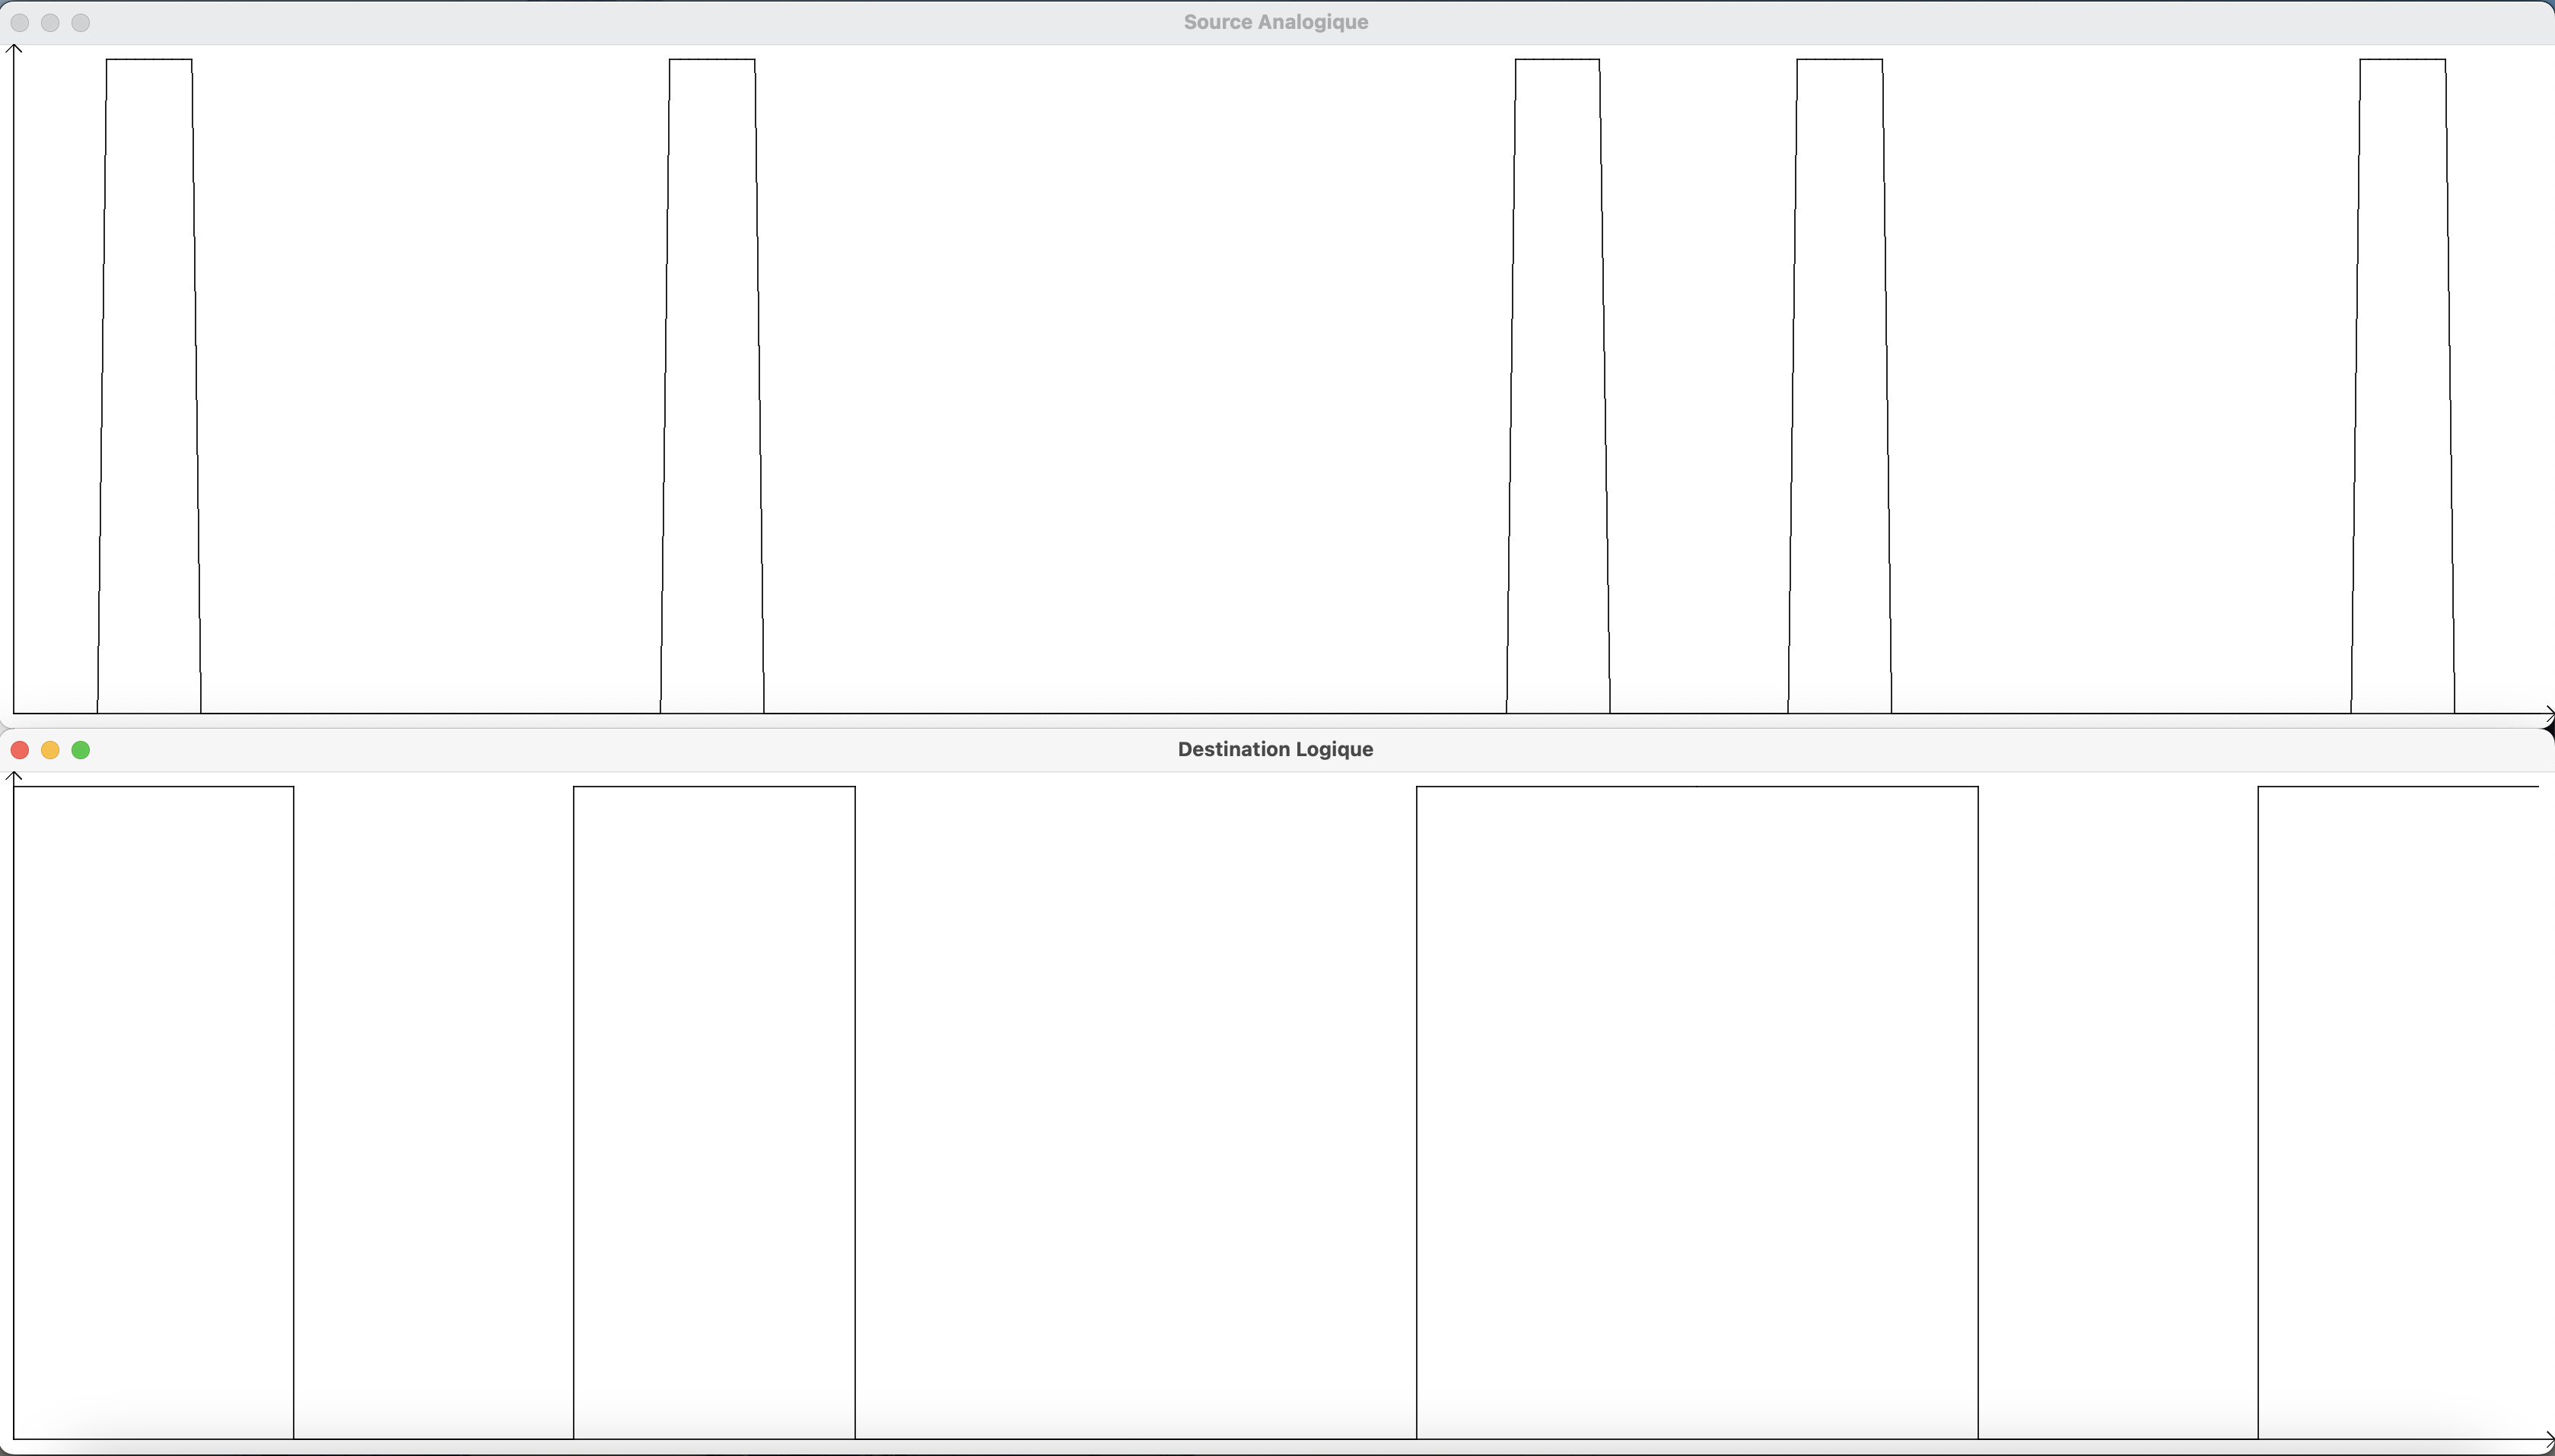
\includegraphics[width=0.5\textwidth]{img/etape2_reception_RZ.png}
    \caption{Réception RZ}
    \label{fig:reception_rz}
\end{figure}

La conversion analogique fonctionne correctement, puisque pour chaque bit à 1, le signal est à son amplitude maximale pendant $\alpha$T et à son amplitude minimale sur (1-$\alpha$)T. Le signal transmis n'étant pas altéré, il s'agit d'un transmetteur analogique parfait. Le TEB est de 0\%.

\subsection{Conclusion étape 2}

Dans cette deuxième étape de notre projet de transmission, nous avons exploré trois méthodes de codage : NRZ, NRZT et RZ, introduisant ainsi une dimension analogique dans notre chaîne de transmission. Nos conclusions montrent que ces méthodes de codage fonctionnent de manière optimale dans des conditions idéales, sans la présence de bruit. 

Le codage NRZ maintient des niveaux stables pour les valeurs binaires 0 et 1, tandis que le NRZT utilise des transitions au milieu de chaque bit pour distinguer efficacement ces valeurs. Enfin, le codage RZ revient à zéro au milieu de chaque période de bit, améliorant la synchronisation entre l'émetteur et le récepteur.

Les tests réalisés montrent que la spécification de chacun de ces trois codages est respectée et nous obtenons des formes de signal conformes aux attentes. Il convient de souligner que, pour l'instant, notre évaluation ne tient pas compte du bruit dans le système, ce qui garantit un taux d'erreur binaire (TEB) de 0\% et une transmission parfaitement fiable. 

\section{TP3 : Transmission bruitée analogique (bruit blanc gaussien)}
\sectionmark{TP3 : Transmission bruitée analogique (bruit blanc gaussien)}

\subsection{Introduction étape 3}

Dans la continuité des étapes 1 et 2, l’objectif principal de cette simulation est d'étudier le comportement du système de transmission lui-même. Cette fois-ci, on prendra en compte une transmission non-idéale avec canal bruité de type \textit{gaussien}. La propagation dans le canal est modélisée de manière théorique par un bruit blanc additif gaussien (AWGN - \textit{Additive white Gaussian noise}) qu’il conviendra de régler en fonction des paramètres du transmetteur vus à l’étape précédente.  


\subsection{Attendus}

Jusqu'alors nous avons implémenté une chaîne de transmission composée d'éléments analogiques et logiques, avec des CAN (Convertisseurs Analogique Numérique) modélisant les codages NRZ, NRZT et RZ. Chaque élément de cette chaîne est dit \textit{parfait}, c'est à dire que la transmission est idéale, sans perte (TEB à 0\%) et sans notion de bruit. Cette étape consistera donc à implémenter du bruit blanc gaussien au niveau du transmetteur, pour modéliser un comportement plus proche de la réalité. Cette section aura vocation à présenter les éléments pris en compte, leur implémentation dans le logiciel et une interprétation physique des résultats obtenus.

Pour apercevoir ces nouvelles implémentations, il faudra utiliser l'option suivante :

Le paramètre \texttt{-snrpb s} permet l'utilisation d’une transmission analogique bruitée, \texttt{s} est la valeur du rapport $\frac{Eb}{N0}$ (en dB). Le paramètre \texttt{s} doit être une valeur flottante. Par défaut, la transmission est non bruitée.

Java n'implémentant pas la loi gaussienne, il nous faudra implémenter celle-ci à partir de lois uniformes. Pour ce faire, nous utilisons la formule suivante :

\vspace{12pt}

$b(n)=\sigma_b\sqrt{-2ln(1-a_1(n))cos(2\pi a_2(n))}$; avec $a_1(n)$ et $a_2(n)$, des lois uniformes et $b(n)$ suivant une loi gaussienne. 

\vspace{12pt}

Dès lors, le signal de sortie sera donné par $s(n)=e(n)+b(n)$, avec $s(n)$ le signal de sortie, $e(n)$ le signal d'entrée et $b(n)$ le bruit blanc gaussien ajouté.

L'implémentation du rapport signal à bruit peut être obtenu de deux manières distinctes (toutes deux homogènes et semblables) :

\vspace{12pt}

\begin{itemize}
    \item $SNR=\frac{P_{signalE}}{P_{bruit}}$ ; Le rapport puissance moyenne du signal émis sur puissance moyenne du bruit.
    \item $\frac{E_b}{N_0}$ ; Le rapport de l'énergie binaire sur la densité spectrale moyenne de bruit.
\end{itemize}

\vspace{12pt}

C'est cette seconde solution qui sera implémentée dans le projet, celle-ci se portant mieux à un contexte de communication binaire. En effet, le rapport $\frac{E_b}{N_0}$ est particulièrement utile pour évaluer la performance des systèmes de communication numérique en termes de taux d'erreur binaire (TEB), celui-ci faisant intervenir la quantité d’échantillons par bit.

\begin{figure}[H]
    \centering
    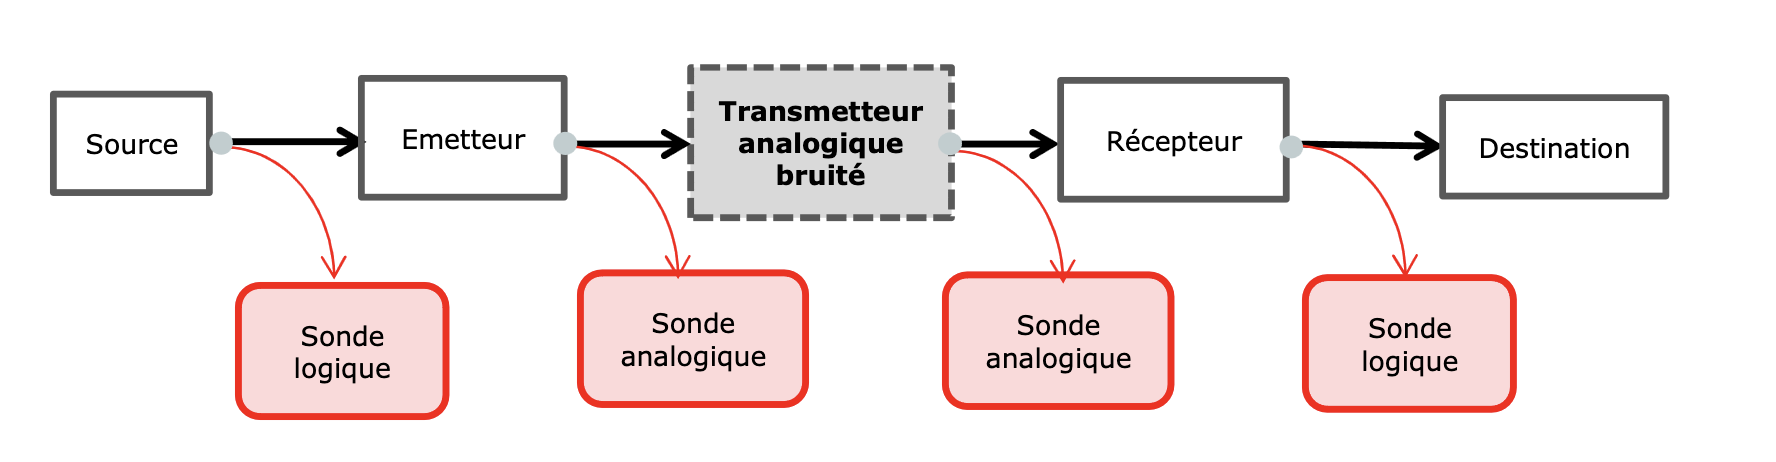
\includegraphics[width=0.9\textwidth]{img/etape2_chaine_transmission_bruitee.png}
    \caption{Chaîne de transmission bruitée}
    \label{fig:chaine_transmission_bruitee}
\end{figure}

\subsection{Réalisation}


\begin{figure}[H]
    \centering
    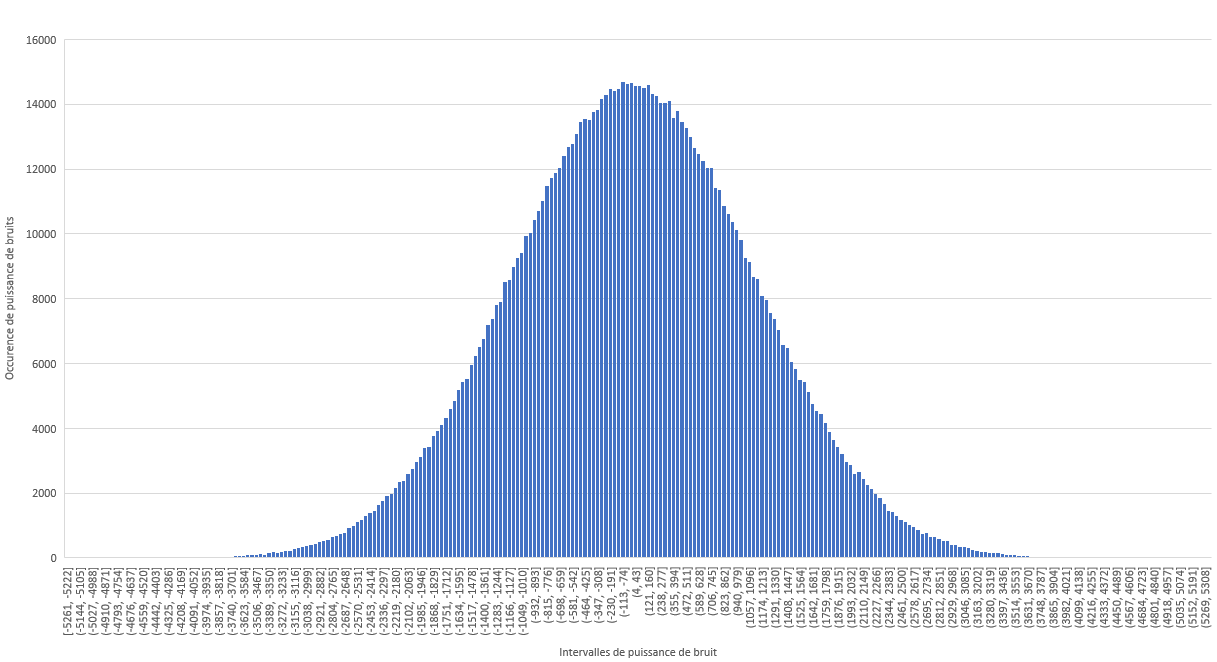
\includegraphics[width=\textwidth]{img/etape3_histo.png}
    \caption{Histogramme de la puissance de bruit moyenne pour 1 000 000 d'échantillons d'un message de 10 bits (NRZ)}
    \label{fig:etape3_histo}
\end{figure}

La répartition des valeurs sur la figure ci-dessus semble très nettement tendre vers une gaussienne (plus le nombre de valeurs sera important, et le pas entre les valeurs faible, plus la définition de cette gaussienne sera importante sur l'histogramme). 

La méthodologie à appliquer pour créer un signal bruité (signal blanc gaussien) étant désormais établie, nous pouvons nous focaliser sur sa mise en oeuvre. Pour cela les éléments suivants ont été implémenté :

Une classe java nommé \textbf{TransmetteurGaussien}, qui reprend le fonctionnement du \textbf{transmetteurParfait} et à laquelle on a ajouté trois méthodes:
     \begin{itemize}
        \item \texttt{calculerPuissanceMoyenneSignal()}
        \item \texttt{calculerVariance()}
        \item \texttt{genererSignalBruite()}
    \end{itemize}

\vspace{20pt}
   
Pour réaliser la méthode \texttt{calculerPuissanceMoyenneSignal()}, reprenons la formule théorique indiquant que la puissance du signal est égale à :

 \begin{align*}
    Ps = \frac{\sum_{i=1}^{k}S(n)^2}{k} 
 \end{align*}

 Nous avons besoin de la puissance du signal émis, pour calculer la valeur de la variance $\sigma_b^2$, car cette dernière nous permet de générer notre bruit en fonction du SNR. On peut obtenir la valeur en renversant l'équation:

\begin{align*}
   SNR =& \frac{P_s * N}{2\sigma b^2}\\
   \sigma_b^2 =& \frac{Ps*N}{2*10^{\frac{SNR}{10}}}\\
\end{align*}
en prenant N le nombre d'échantillon et Ps la puissance du signal

On obtient alors la valeur de $\sigma$:
\begin{align*}
 \sigma_b =& \sqrt{\frac{Ps*N}{2*10^{\frac{SNR}{10}}}}\\
\end{align*}

À partir de la valeur trouvé ci-dessous, on peut désormais générer notre bruit blanc gaussien pour réaliser le transmetteur bruité. Grâce à l'étape deux et aux calculs ci-dessus, on peut modéliser le passage d'un bruit blanc gaussien à travers différents types de codage (RZ, NRZ, NRZT) :

\subsubsection{Émission analogique RZ d'un signal bruité}
\begin{figure}[H]
    \centering
    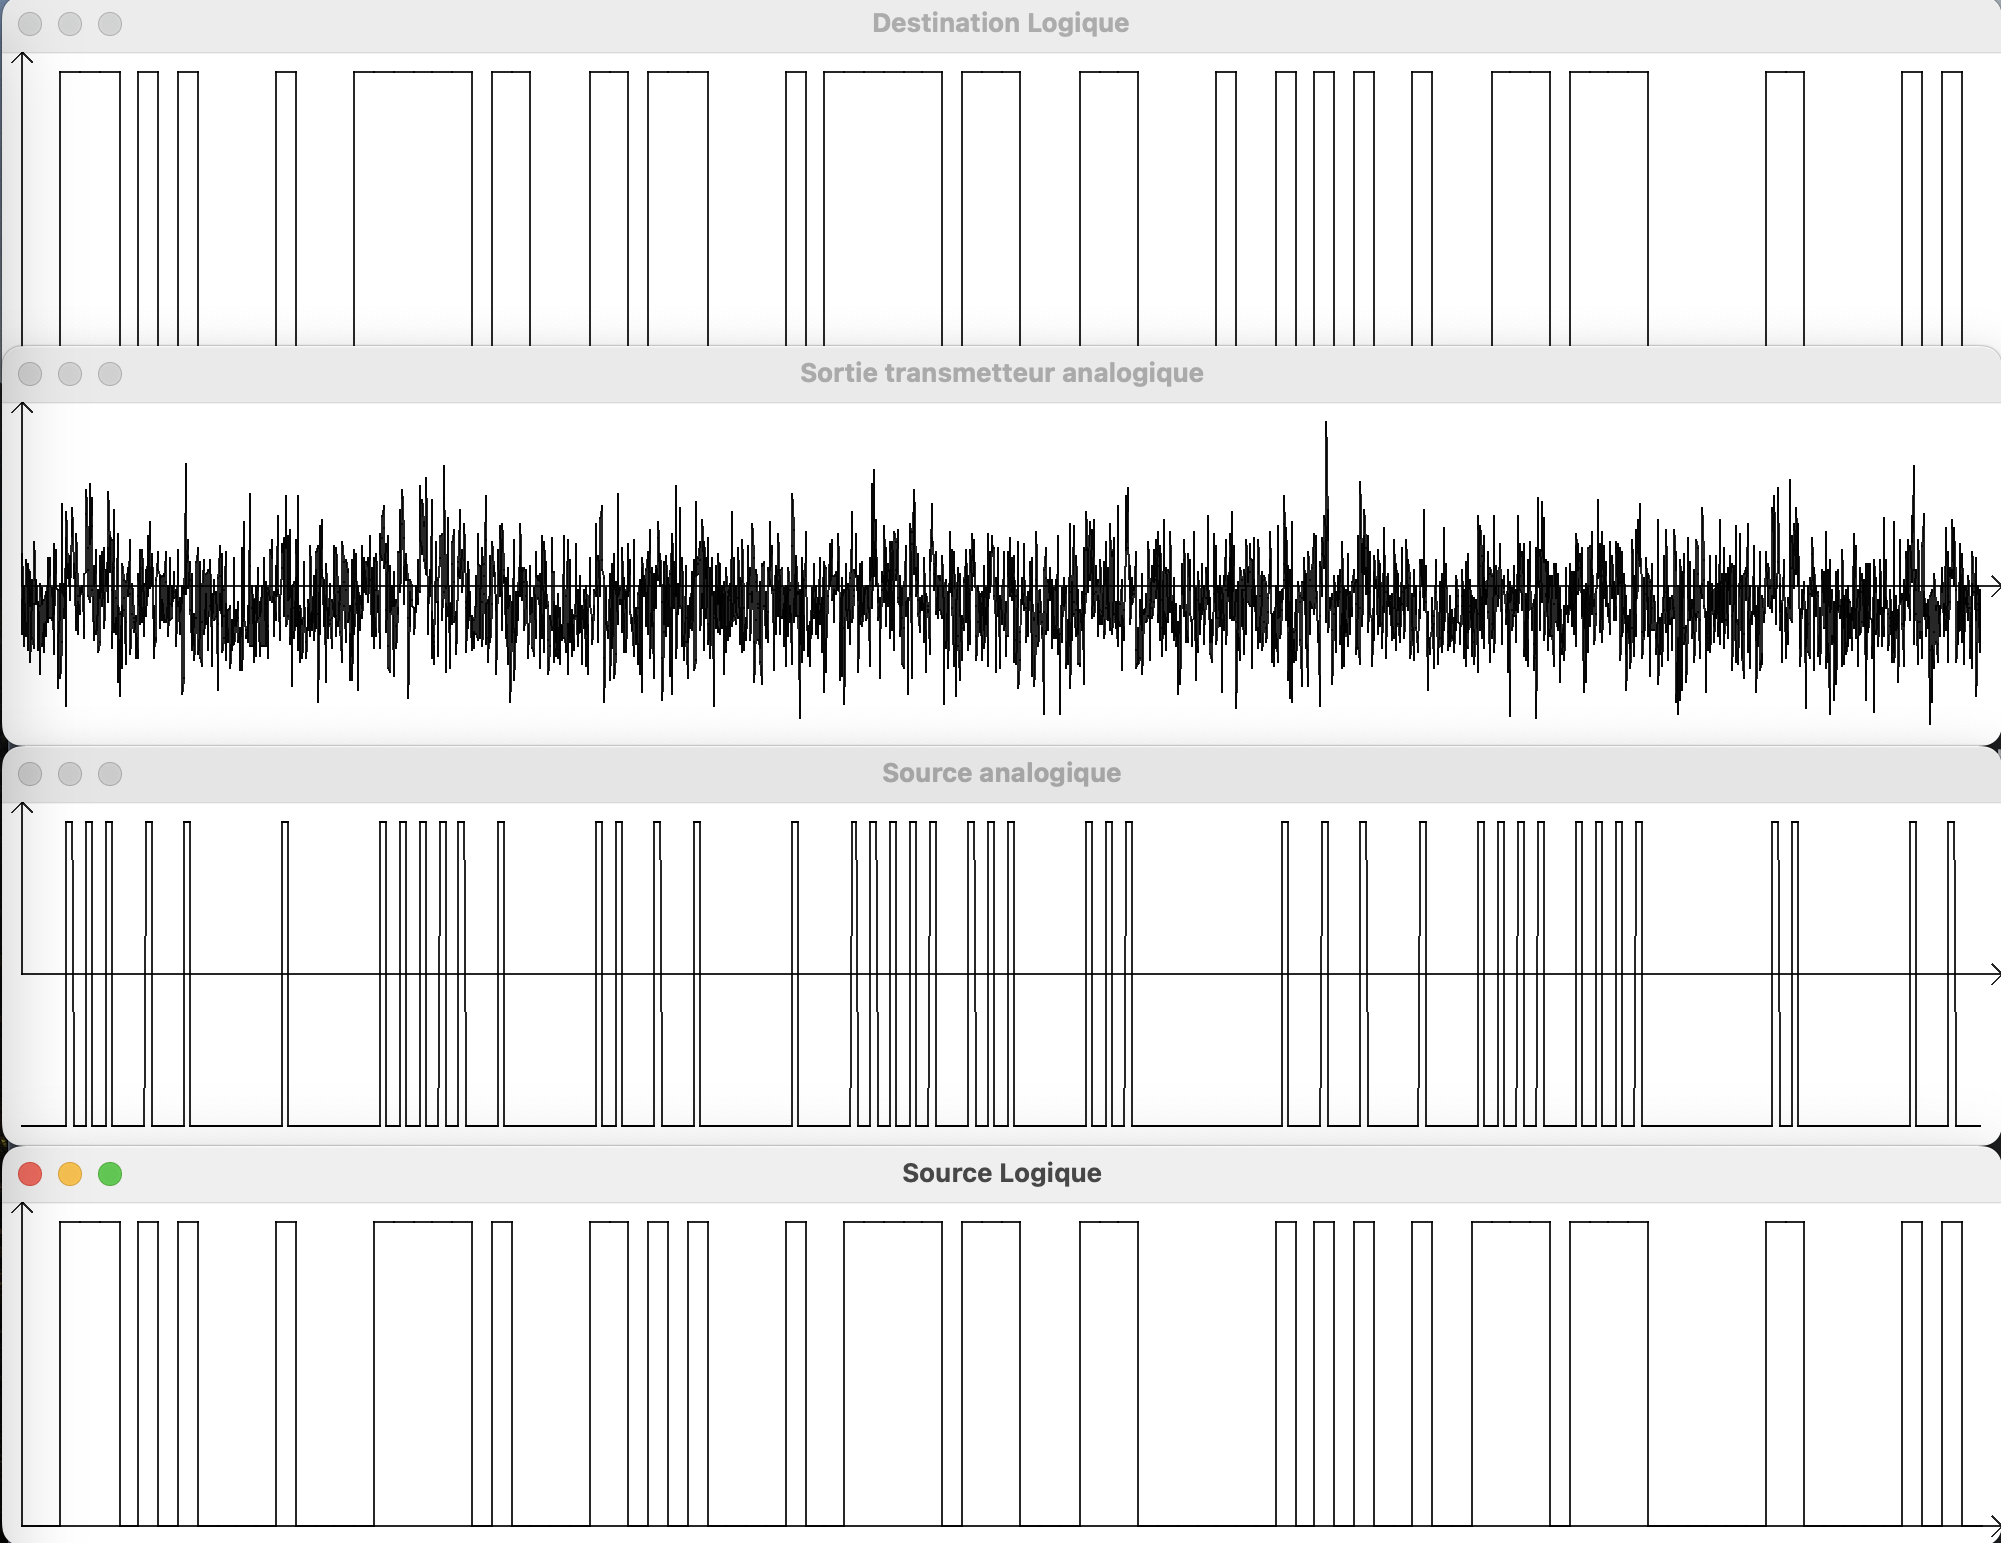
\includegraphics[width=0.7\textwidth]{img/etape3_emission_RZ_bruite.png}
    \caption{Graphe des sondes de la chaîne de transmission pour un message de 100 bits de forme RZ et pour un SNR de 5 }
    \label{fig:etape_3_RZ_bruite}
\end{figure}

On réalise la simulation d'un signal bruité RZ de 100 bits et un SNR de 5. D'après ce que l'on a déjà simulé à l'étape 2, on observe bien au niveau de la sonde pour l'émission analogique, chaque changement de valeur d'un bit logique est suivi d'un passage par l'état 0. Pour ce qui est du transmetteur bruité, on remarque très clairement l'ajout de bruit au signal d'origine. Cela va entraîner des erreurs à la sortie du transmetteur, on voit notre TEB a une valeur de 0.06.

\begin{figure}[H]
    \centering
    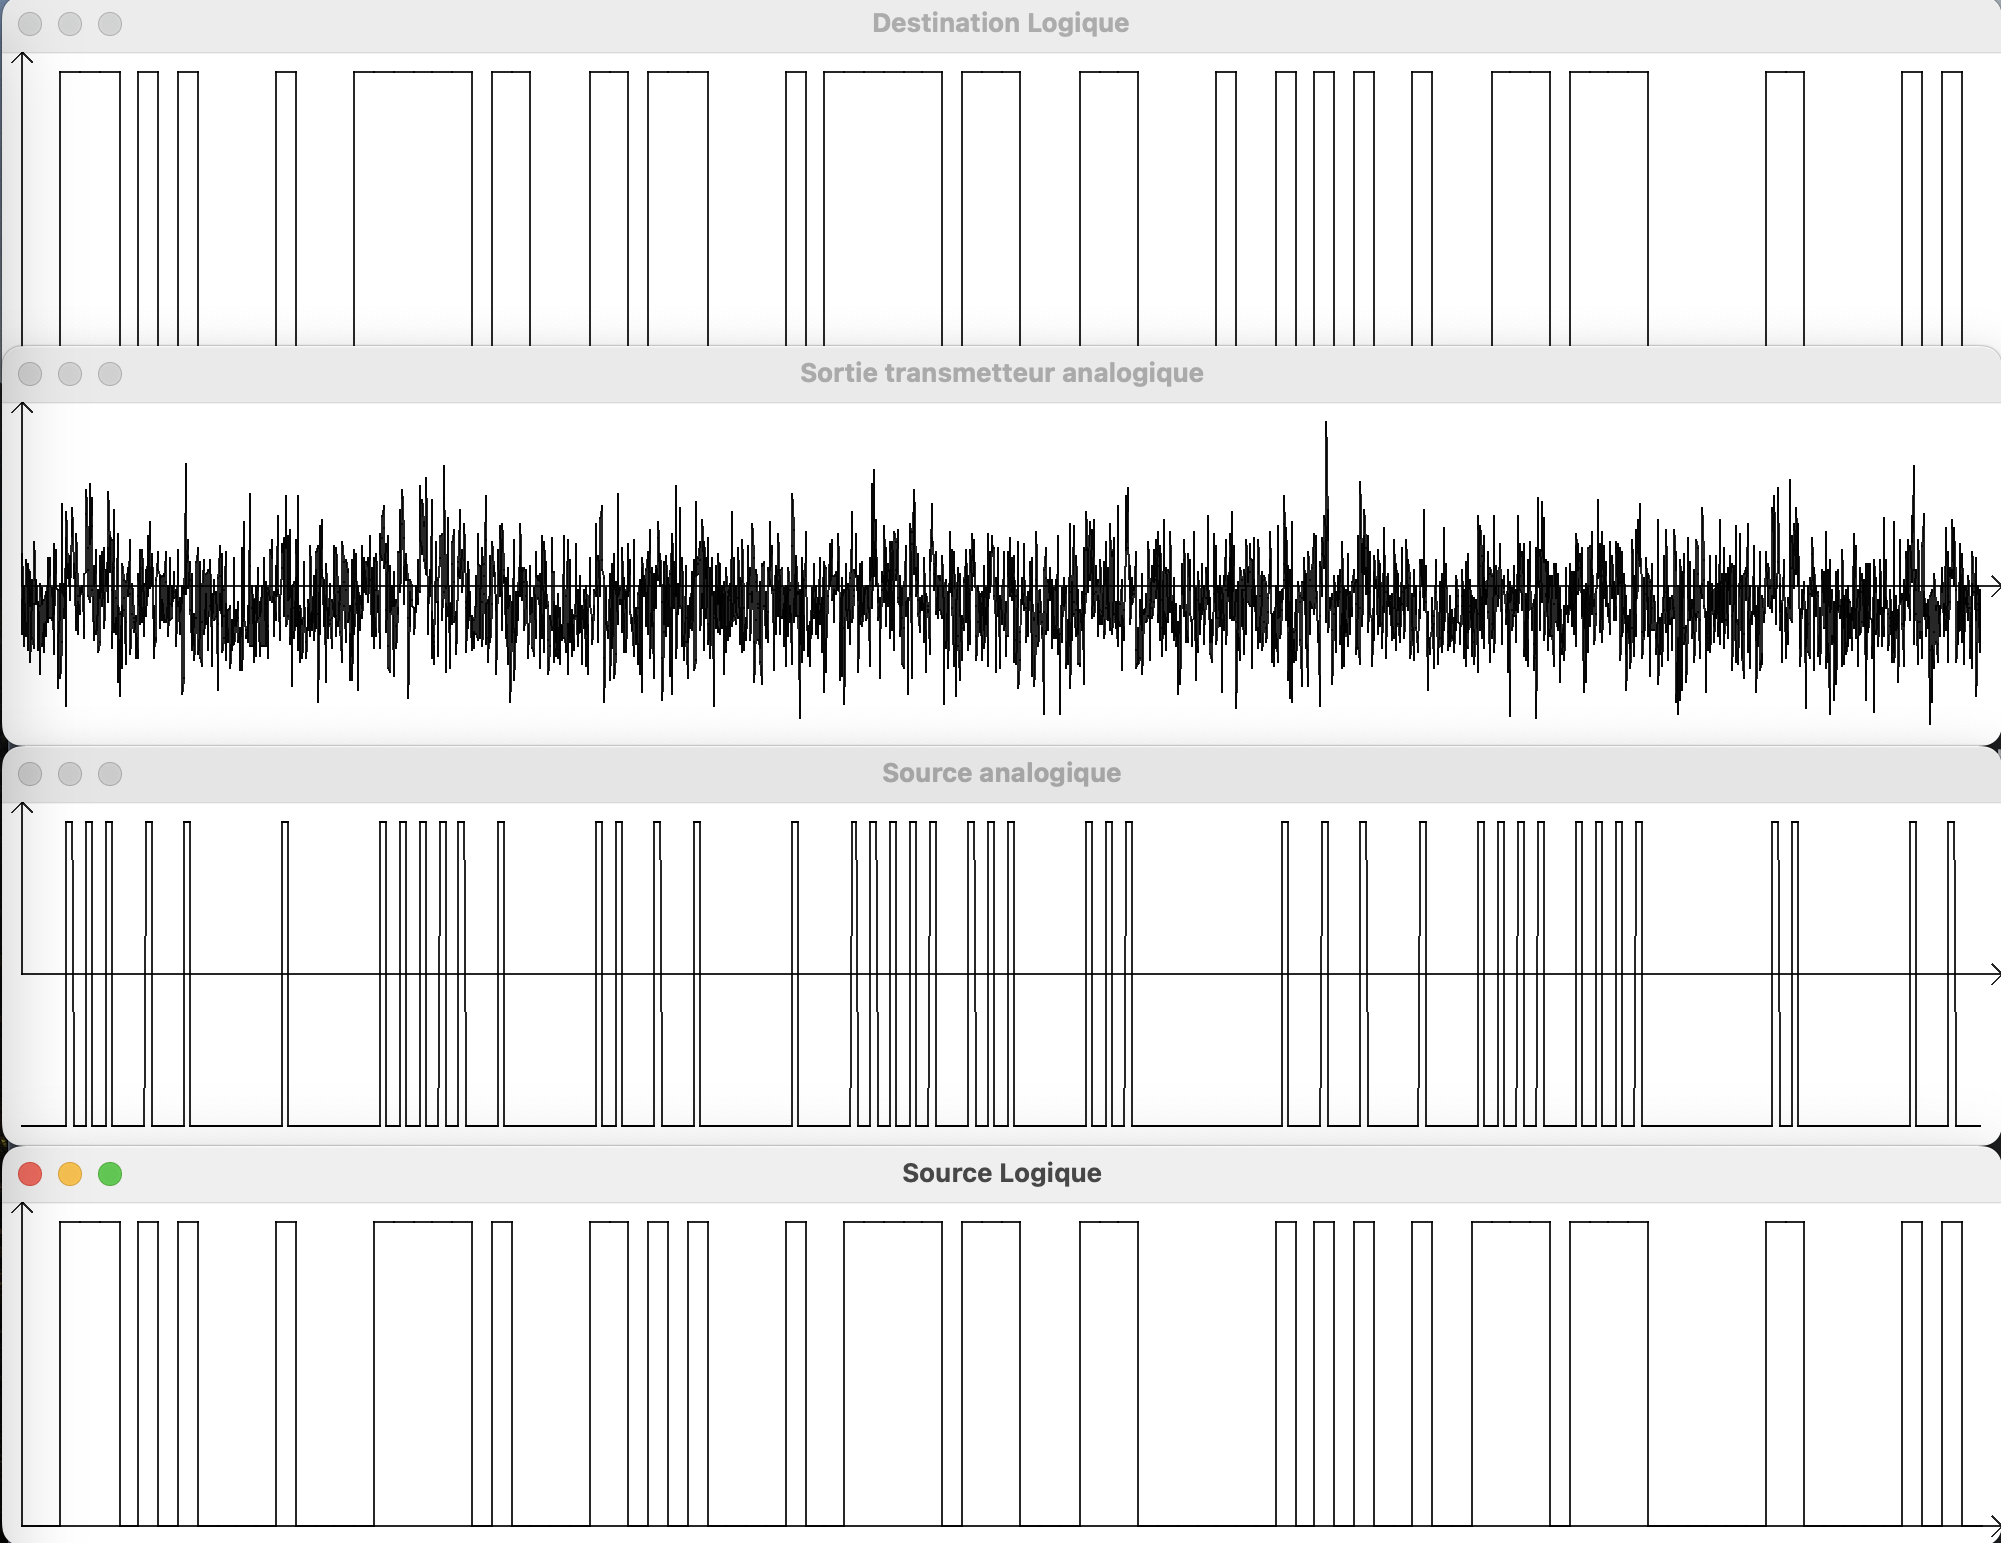
\includegraphics[width=0.7\textwidth]{img/etape3_emission_RZ_bruite.png}
    \caption{Graphe montrant l'évolution du TEB en fonction du SNR pour un signal RZ }
    \label{fig:etape_3_RZ_bruite}
\end{figure}

L'observation que l'on peut faire de ce graphe est que la valeur du TEB va tendre vers 0.5 lorsque l'on a une valeur de SNR augmente dans les négatifs. Au contraire lorsque le SNR augmente dans les positifs, la valeur du TEB diminue, et tend vers 0. Il y a une probabilité assez importante d'avoir une erreur de codage du signal.


\subsubsection{Émission analogique NRZ d'un signal bruité}

\begin{figure}[H]
    \centering
    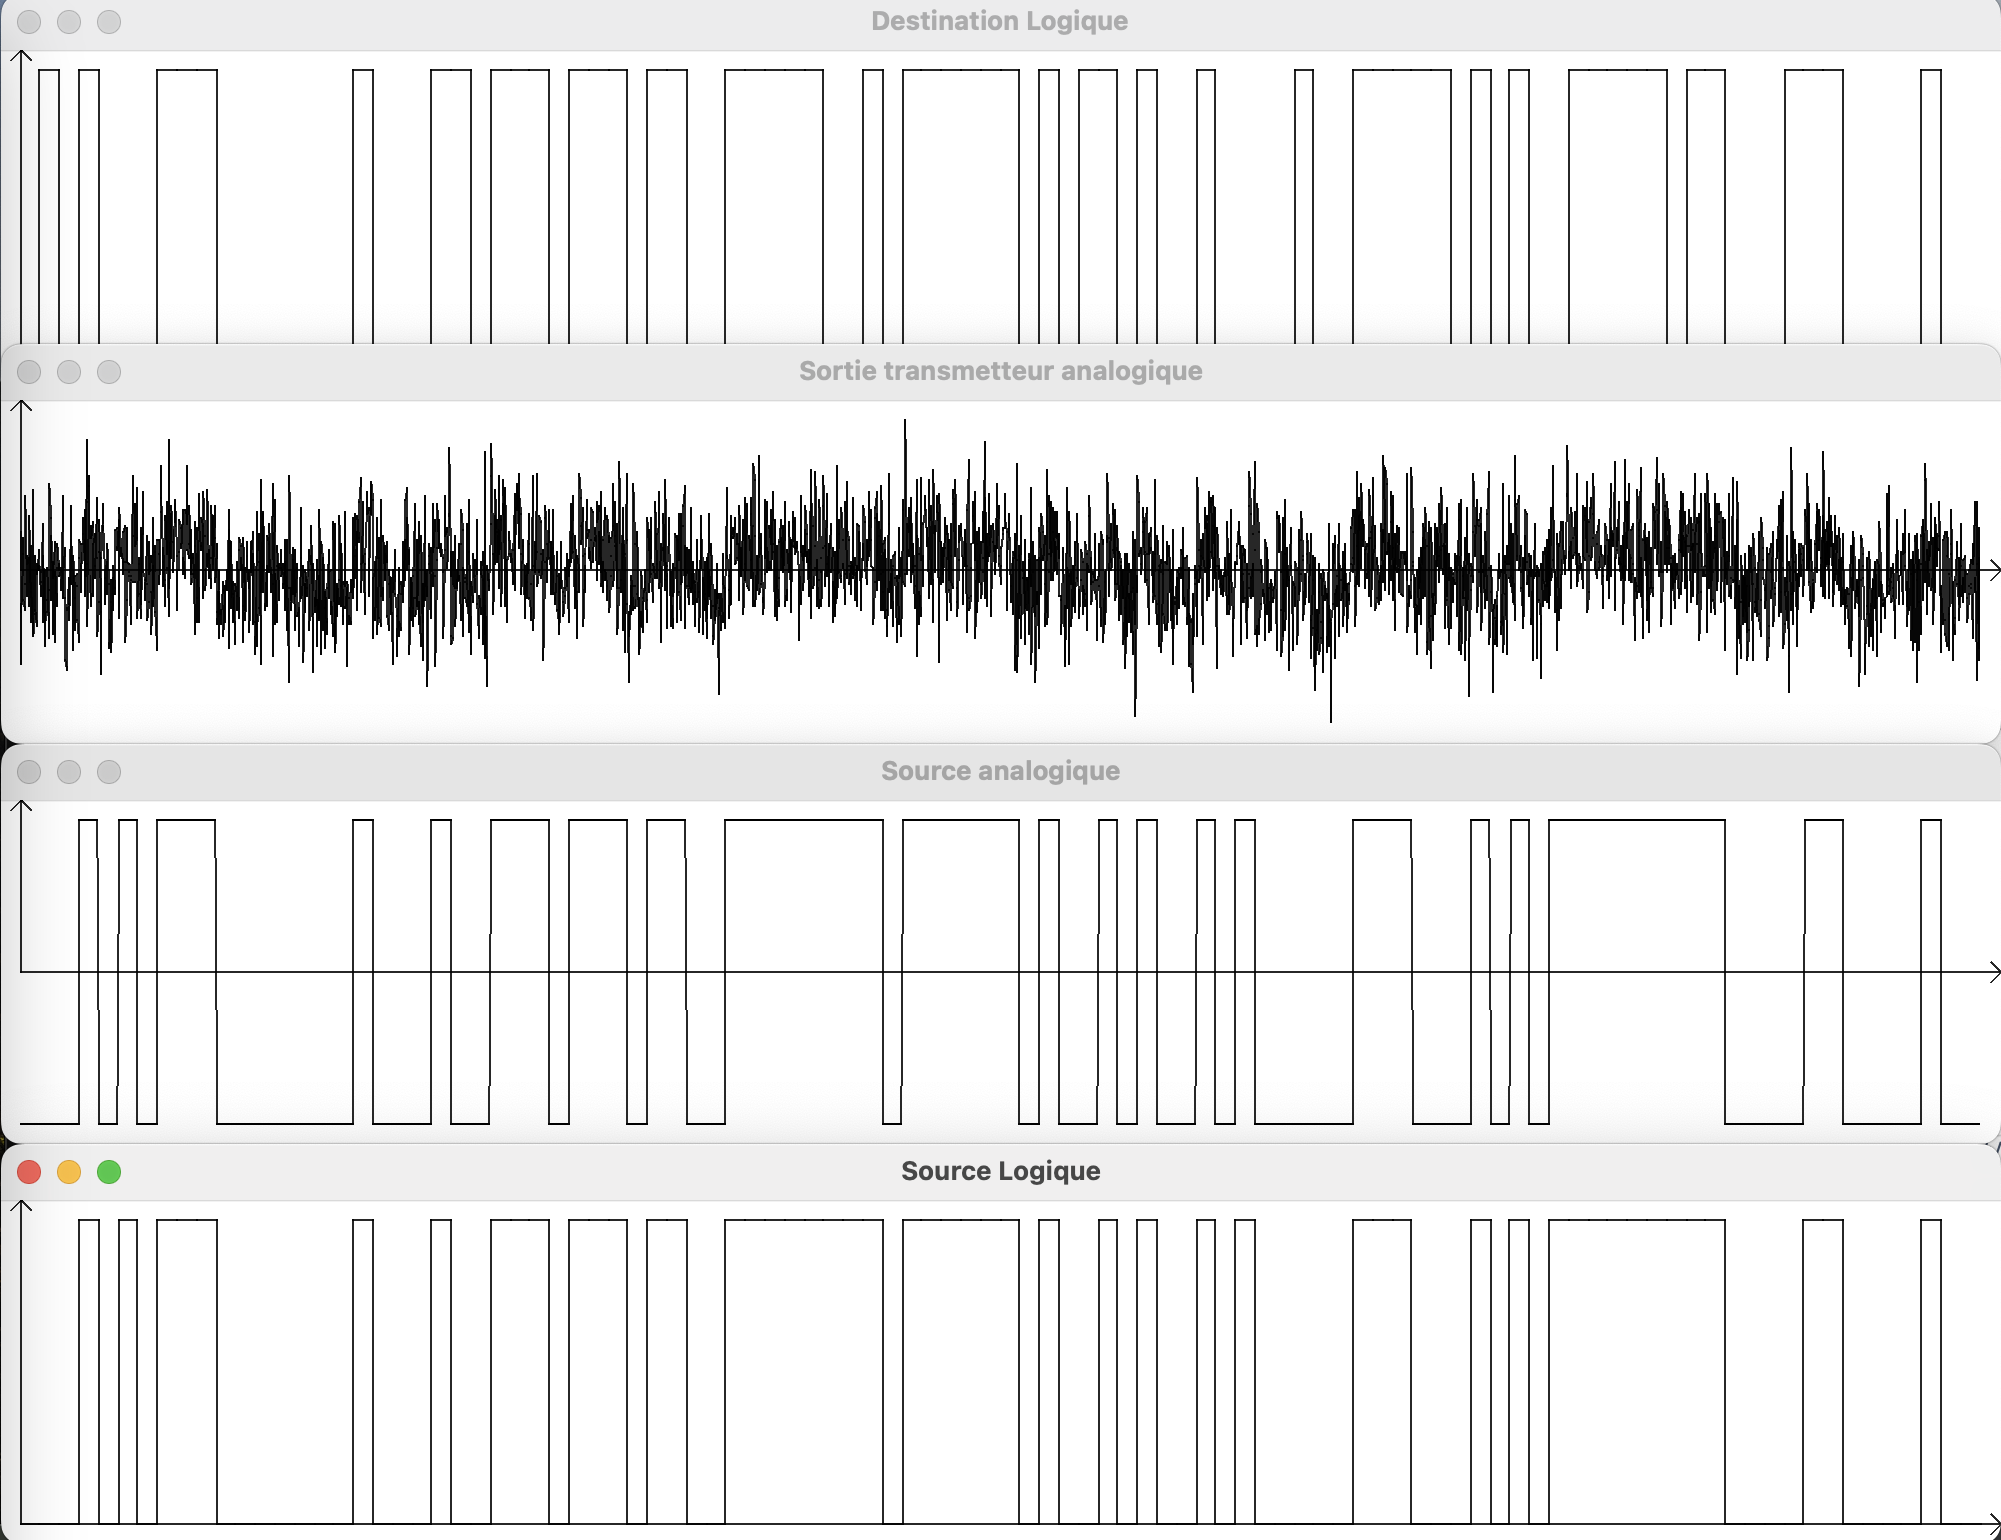
\includegraphics[width=0.7\textwidth]{img/etape3_emission_NRZ_bruite.png}
    \caption{Graphe des sondes de la chaîne de transmission pour un message de 100 bits de forme NRZ et pour un SNR de 5 db}
    \label{fig:etape_3_NRZ_bruite}
\end{figure}

On réalise la simulation d'un signal bruité NRZ de 100 bits et un SNR de 5. D'après ce que l'on a généré pour l'étape 2, on remarque bien les caractéristique du signal NRZ sur la simulation. En effet, on a bien un signal codé à l'aide de deux états, sans état intermédiaire. Pour ce qui est du transmetteur bruité, on remarque très clairement l'ajout de bruit au signal d'origine. Notamment, aux niveaux des amplitudes du signal, on observe une variation importante après l'ajout du bruit. C'est la cause de l'augmentation du TEB, l'ajout de bruit fait parfois dépasser le seuil de détection du symbole, ce qui peut empêcher la récupération du message côté récepteur. Ce phénomène est visible sur la simulation car on obtient un TEB de 0.19.

\begin{figure}[H]
    \centering
    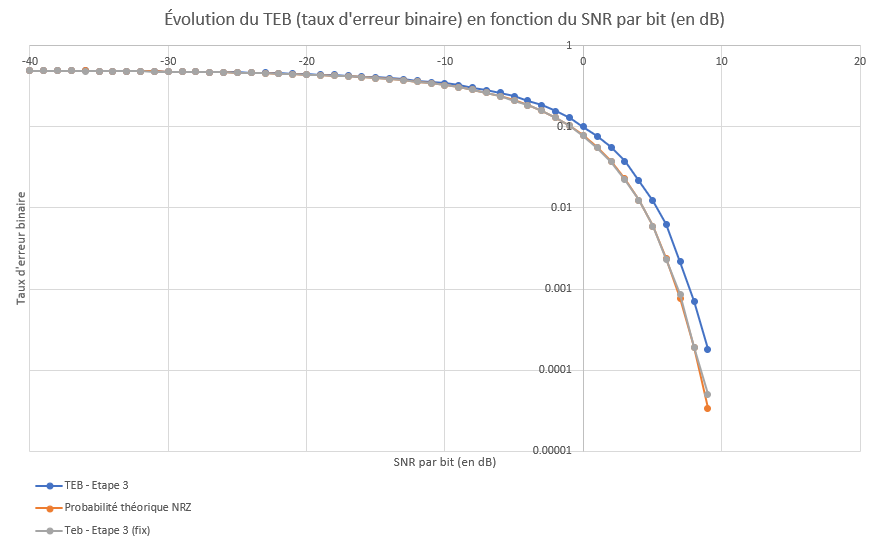
\includegraphics[width=0.8\textwidth]{img/etape3_teb_fct_snr.png}
    \caption{Tracé du TEB en fonction du SNR par bit (semence constante, message de 100000 symboles, codage NRZ, 30 échantillons par symbole)}
    \label{fig:etape3_teb_fct_snr}
\end{figure}

L'analyse de la courbe ci-dessus met en évidence une relation significative entre le rapport signal sur bruit ($\frac{E_B}{N_0}$) et le taux d'erreur binaire (TEB/BER). En effet, lorsque le rapport signal sur bruit est faible, le TEB augmente considérablement, ce qui reflète la sensibilité du signal à un environnement bruité. À l'inverse, lorsque le SNR est élevé, le bruit a moins d'impact, ce qui se traduit par une réduction du TEB. Il convient d'observer les courbes théoriques de chaque type de modulation et de les comparer aux résultats expérimentaux de notre système.

\subsubsection{Émission analogique NRZT d'un signal bruité}
\begin{figure}[H]
    \centering
    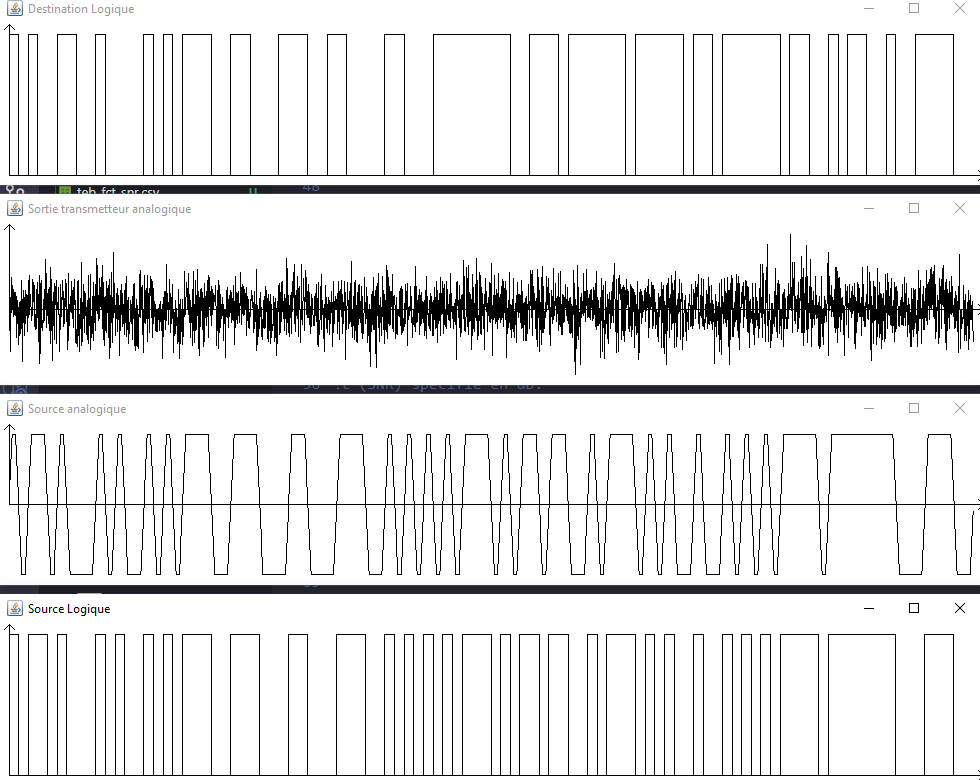
\includegraphics[width=0.7\textwidth]{img/etape3_emission_NRZT_bruite.png}
    \caption{Graphe des sondes de la chaîne de transmission pour un message de 100 bits de forme NRZT et pour un SNR de 5}
    \label{fig:etape_3_NRZT_bruite}
\end{figure}

On réalise la simulation d'un signal bruité NRZT de 100 bits et un SNR de 5. D'après ce que l'on a déjà simulé à l'étape 2, on observe bien au niveau de la sonde pour l'émission analogique, chaque changement de valeur d'un bit logique est réalisé de manière progressive, on voit bien une pente pour la montée et descente du symbole. Pour ce qui est du transmetteur bruité, on remarque très clairement l'ajout de bruit au signal d'origine. Cela va entraîner des erreurs à la sortie du transmetteur, on voit notre TEB a une valeur de 0.167.

\begin{figure}[H]
    \centering
    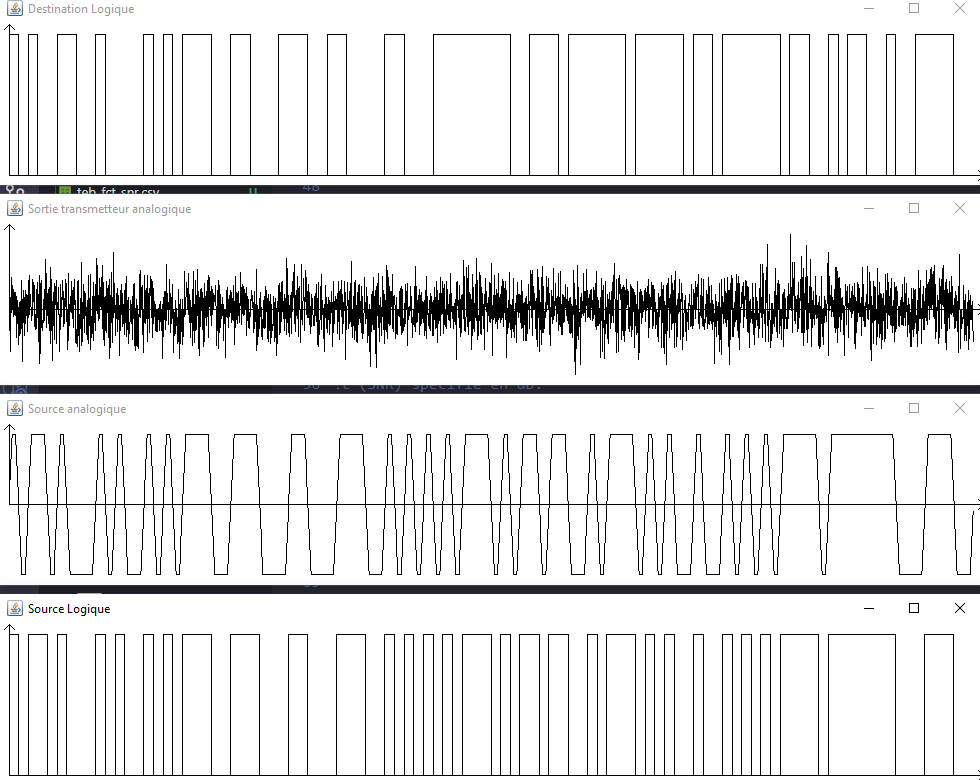
\includegraphics[width=0.7\textwidth]{img/etape3_emission_NRZT_bruite.png}
    \caption{Tracé du TEB en fonction du SNR par bit (semence constante, message de 100000 symboles, codage TNRZ, 30 échantillons par symbole)}
    \label{fig:etape_3_NRZT_bruite}
\end{figure}

L'analyse de la courbe ci-dessus met en évidence une relation significative entre le rapport signal sur bruit ($\frac{E_B}{N_0}$) et le taux d'erreur binaire (TEB/BER). En effet, lorsque le rapport signal sur bruit est faible, le TEB augmente considérablement, ce qui reflète la sensibilité du signal à un environnement bruité. À l'inverse, lorsque le SNR est élevé, le bruit a moins d'impact, ce qui se traduit par une réduction du TEB. Il convient d'observer les courbes théoriques de chaque type de modulation et de les comparer aux résultats expérimentaux de notre système.


\subsection{Conclusion étape 3}

En conclusion, nous avons réussi à introduire un élément essentiel à la modélisation d'une chaîne de transmission : un canal de transmission analogique bruité. Ce canal a été conçu pour simuler les conditions réelles auxquelles les signaux sont confrontés lors de leur transmission dans un environnement physique, pour lequel la modélisation sous forme de bruit blanc gaussien prend sens (théorème central limite). Le paramètre clé ici est le rapport signal sur bruit ($\frac{E_B}{N_0}$), qui joue un rôle déterminant dans la qualité de la transmission.

\section*{Annexes}
\sectionmark{Annexes}
\addcontentsline{toc}{section}{Annexes}

\subsection{Trace de l'exécution des tests au 7 septembre}
\begin{figure}[H]
    \centering
    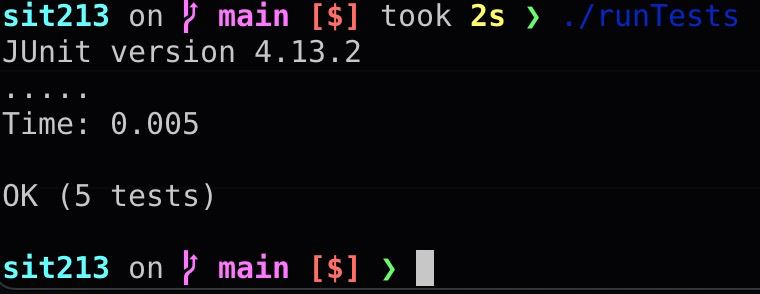
\includegraphics[width=\textwidth]{img/runTests.jpg}
    \caption{Résultat de l'exécution des tests JUnit}
    \label{fig:tests1}
\end{figure}


\end{document}
